\documentclass[10pt,twocolumn,letterpaper]{article}

\usepackage{cvpr}
\usepackage{times}
\usepackage{epsfig}
\usepackage{graphicx}
\usepackage{amsmath}
\usepackage{amssymb}
\usepackage{float} 
\usepackage{subfigure} 
\usepackage{bm} 
\usepackage{algorithm}
\usepackage{tabularx}
\usepackage{algpseudocode}
\usepackage{subfloat}
\usepackage{verbatim}


\usepackage[pagebackref=true,breaklinks=true,letterpaper=true,colorlinks,bookmarks=false]{hyperref}
\usepackage[american]{babel}
\usepackage{microtype}

\hypersetup{
    colorlinks=true,
    linkcolor=blue,
    filecolor=red,      
    urlcolor=red,
    citecolor=green,
}

\makeatletter
\usepackage{xspace}
\DeclareRobustCommand\onedot{\futurelet\@let@token\@onedot}
\def\@onedot{\ifx\@let@token.\else.\null\fi\xspace}
\def\eg{\emph{e.g}\onedot}
\def\ie{\emph{i.e}\onedot}
\def\etal{\emph{et al}\onedot}
\makeatother

\def\cvprPaperID{6791}

\def\httilde{\mbox{\tt\raisebox{-.5ex}{\symbol{126}}}}

\renewcommand{\algorithmicrequire}{\textbf{Input:}}
\renewcommand{\algorithmicensure}{\textbf{Output:}}

\begin{document}

\bibliographystyle{plain}


\title{Learning to Cartoonize Using White-box Cartoon Representations\\Supplementary Material}
\maketitle

\begin{figure*}[b]
\centering
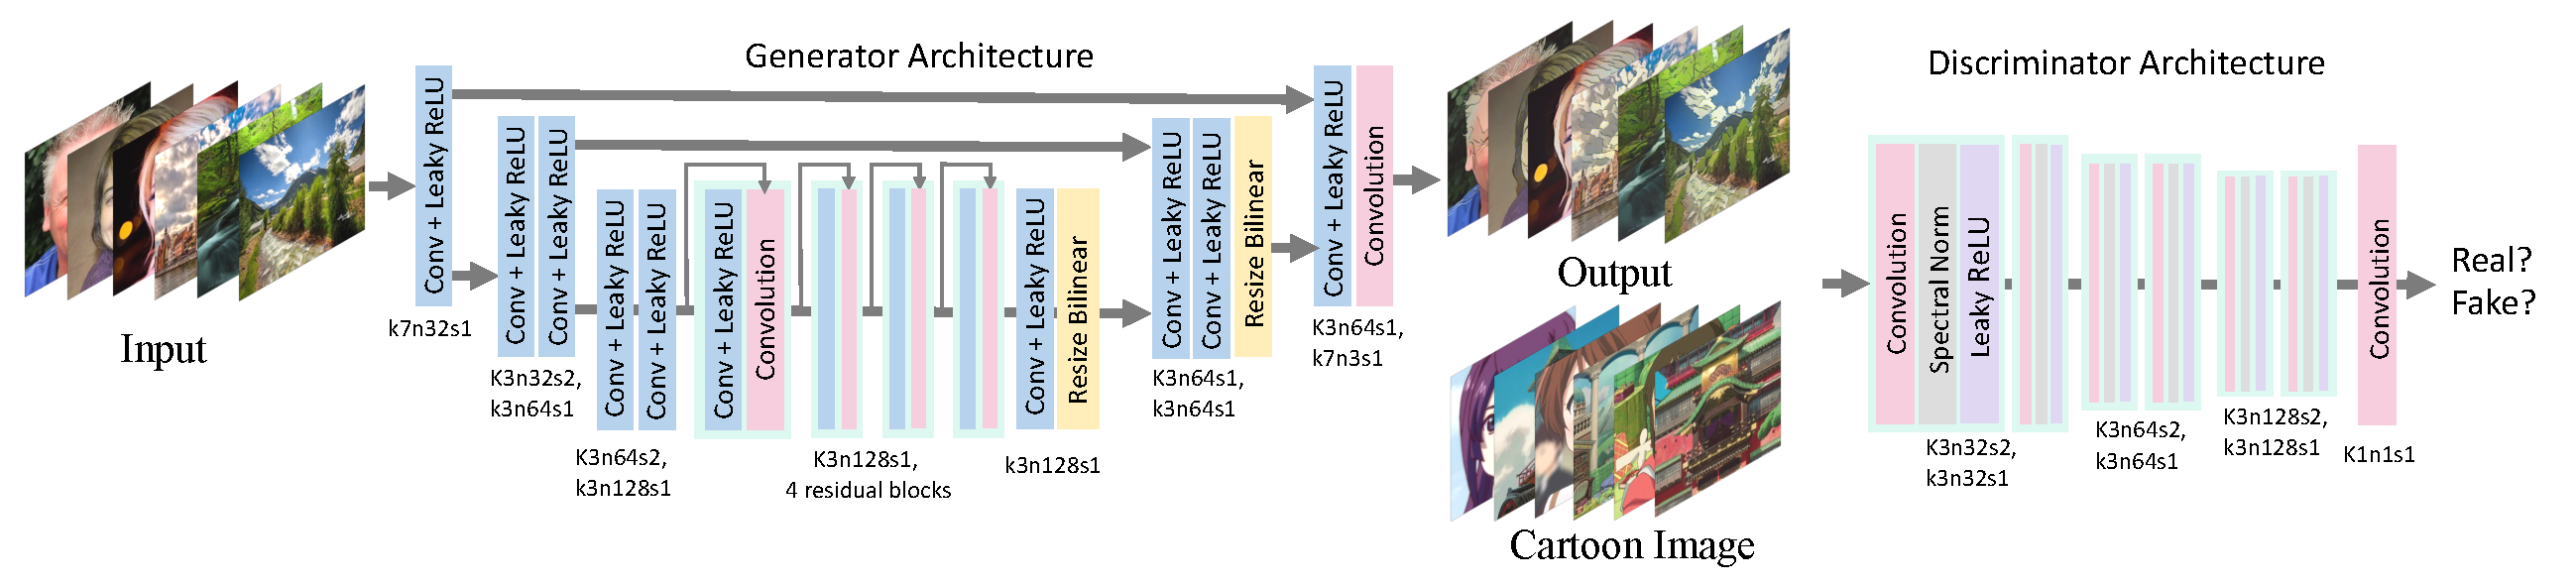
\includegraphics[width=\linewidth]{figures/network_architecture.pdf}
\caption{The architecture of generator network and discriminator network.}
\label{fig:network_architecture}
\end{figure*}

\section{Overview}
In this supplementary material, we show more experimental results, including the architecture of generator network and discriminator network, the influence of different loss functions in generative adversarial networks (GANs), illustration of our method in different scenes with different style, and examples used in the user study.

\section{Network Architecture}
We show the architecture of generator network and discriminator network in Figure \ref{fig:network_architecture}. The generator network is a fully-convolutional network consisted of only convolution, activation and bilinear-resize layers, which enables it to be easily embedded in edge devices such as mobile phones. PatchGAN \cite{isola2017image} is adapted in the discriminator network, where the last layer is a convolution layer. Each pixel in the output feature map correspond to a patch in the input image, with the size equals to the perceptive field, and is used to judge whether the patch belongs cartoon images or generated images. Spectral normalization \cite{miyato2018spectral} is placed after every convolution layer (except the last one) to enforce the Lipschitz constrain on the network and stabilize training. 


\section{Influence of Different GAN loss}
In our proposed framework, least square GAN (LSGAN) loss \cite{mao2017least} is used for adversarial training. We also tested the vanilla GAN loss \cite{goodfellow2014generative}, Wasserstein GAN loss with gradient-penalty \cite{gulrajani2017improved}, and LSGAN loss with spectral norm removed in discriminator. The results of different gan loss are shown in Figure \ref{}.

\section{Influence of Different GAN loss}

\begin{figure*}[b]
\vspace{-0.5em}
\centering
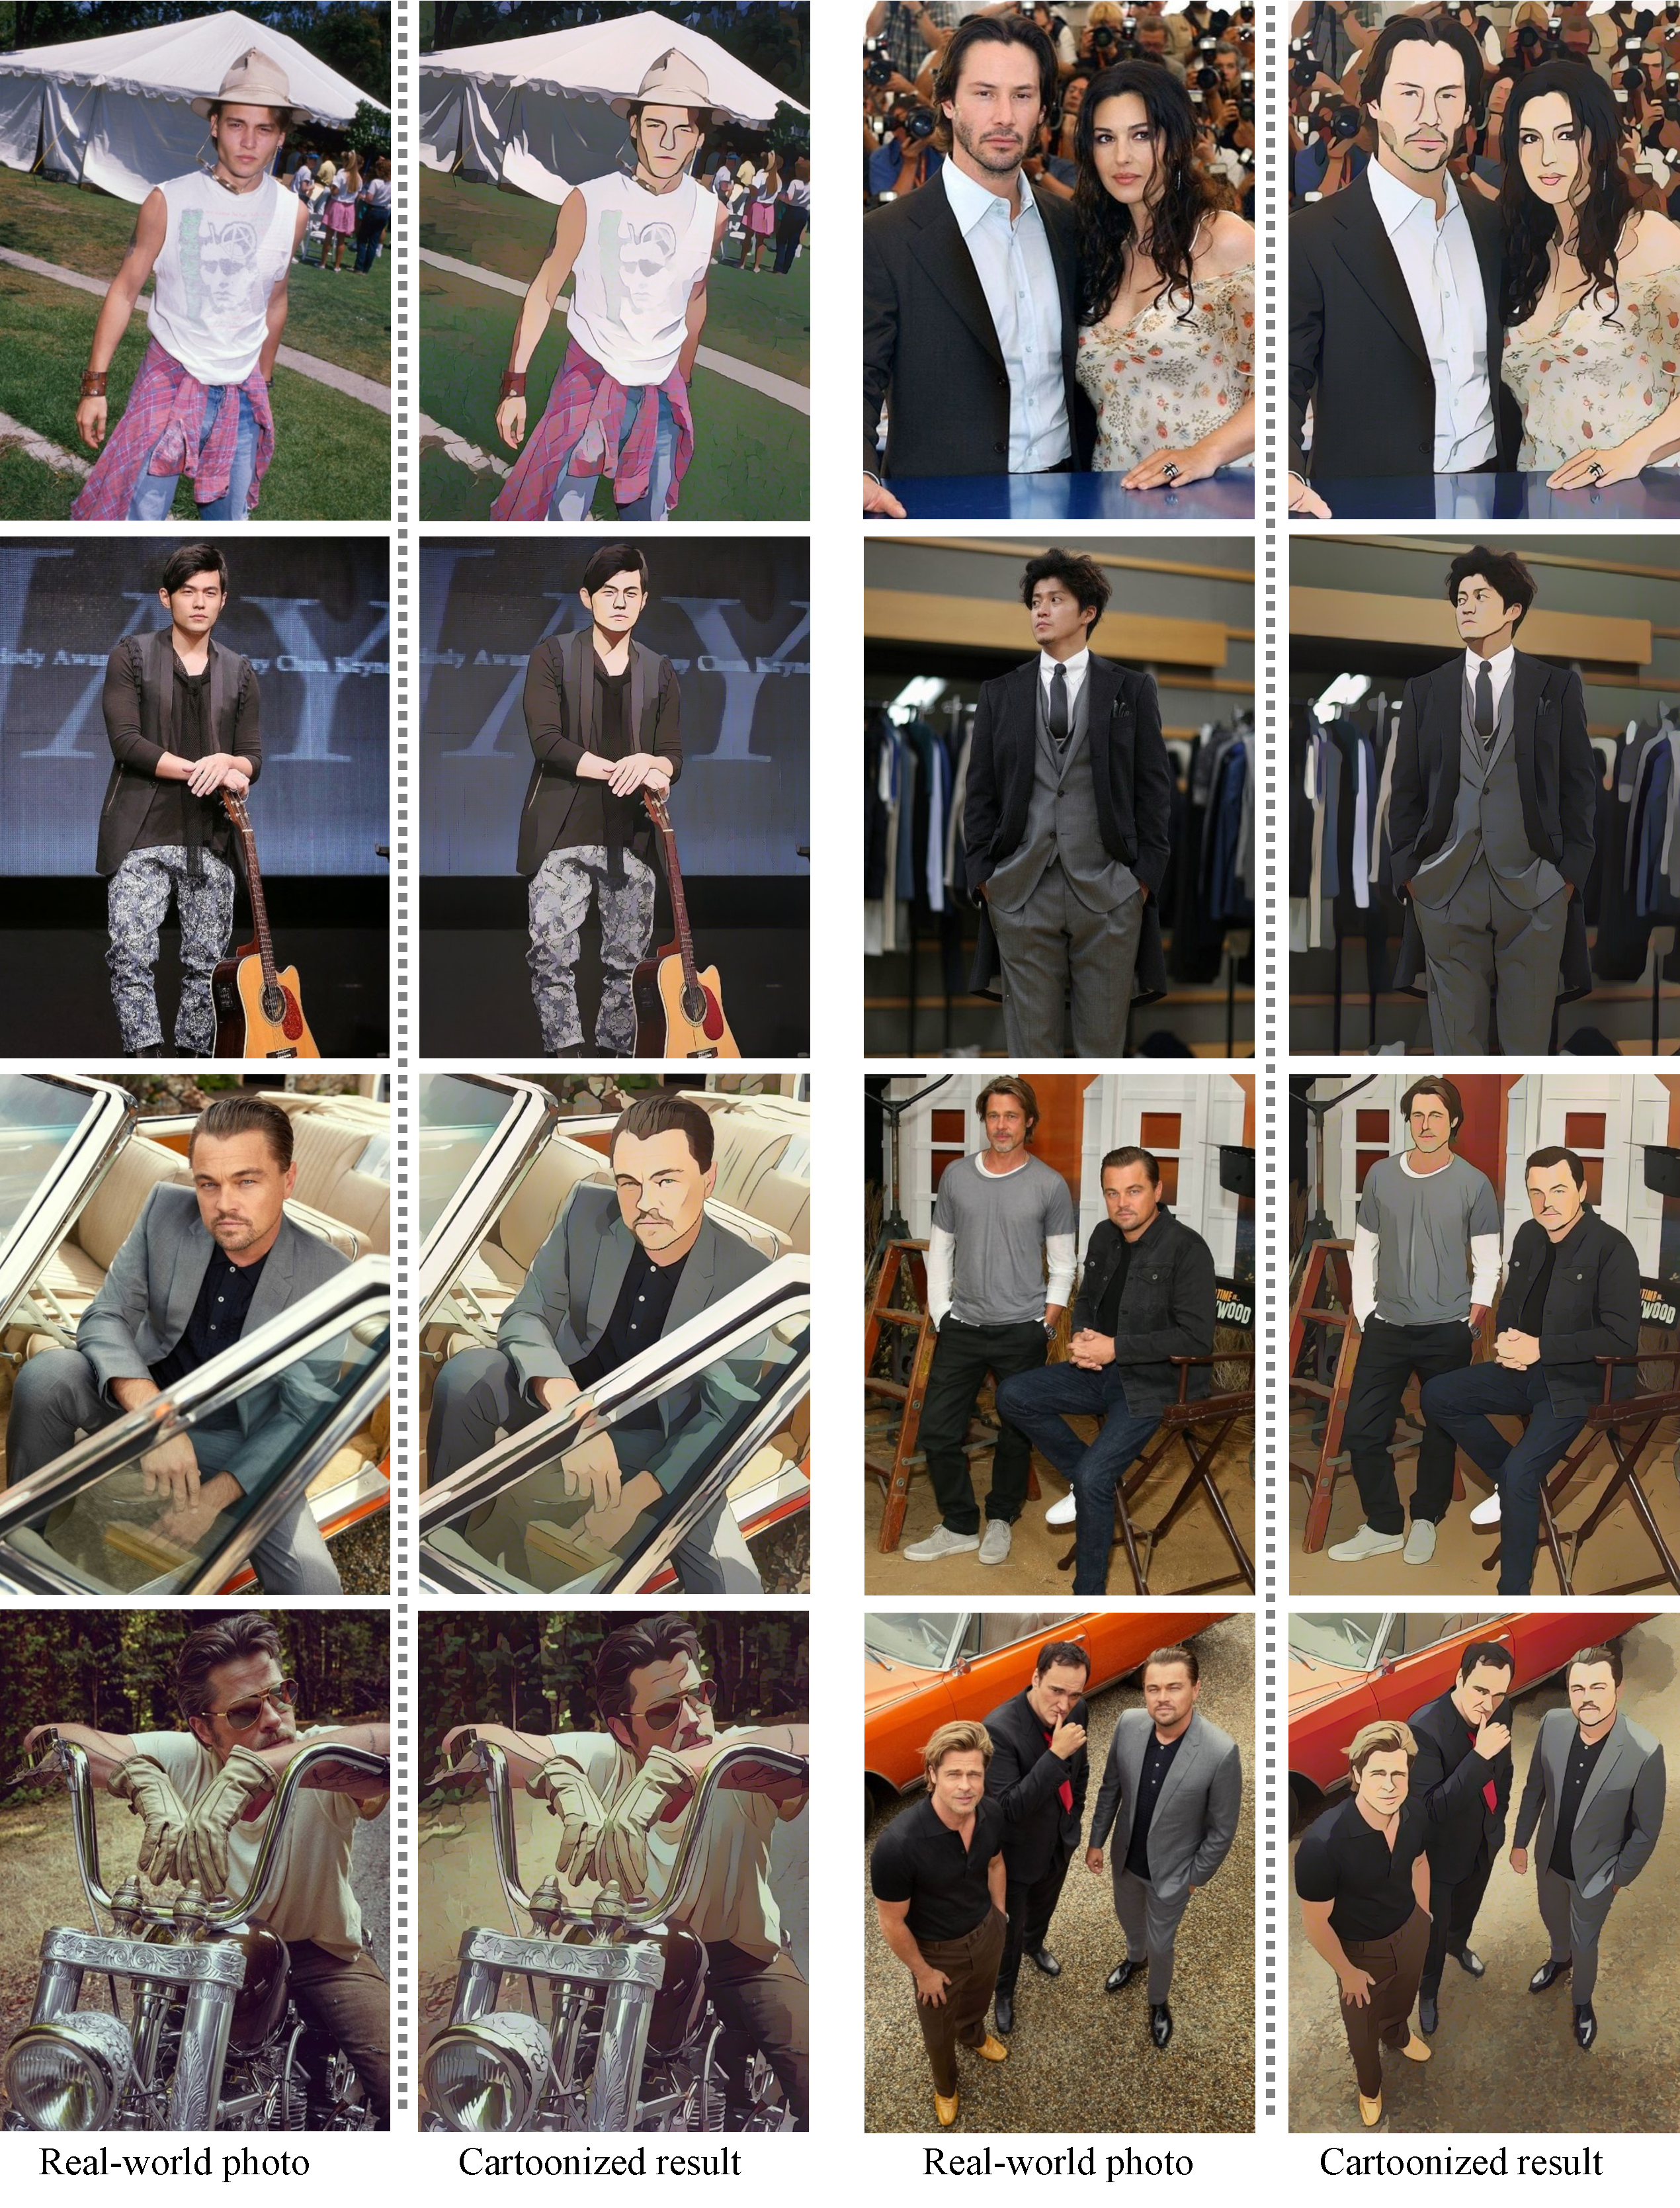
\includegraphics[width=\linewidth]{figures/person1.pdf}
\caption{Cartoonized male Celebrities.}
\label{fig:person1}
\vspace{-0.5em}
\end{figure*}

\begin{figure*}[b]
\vspace{-0.5em}
\centering
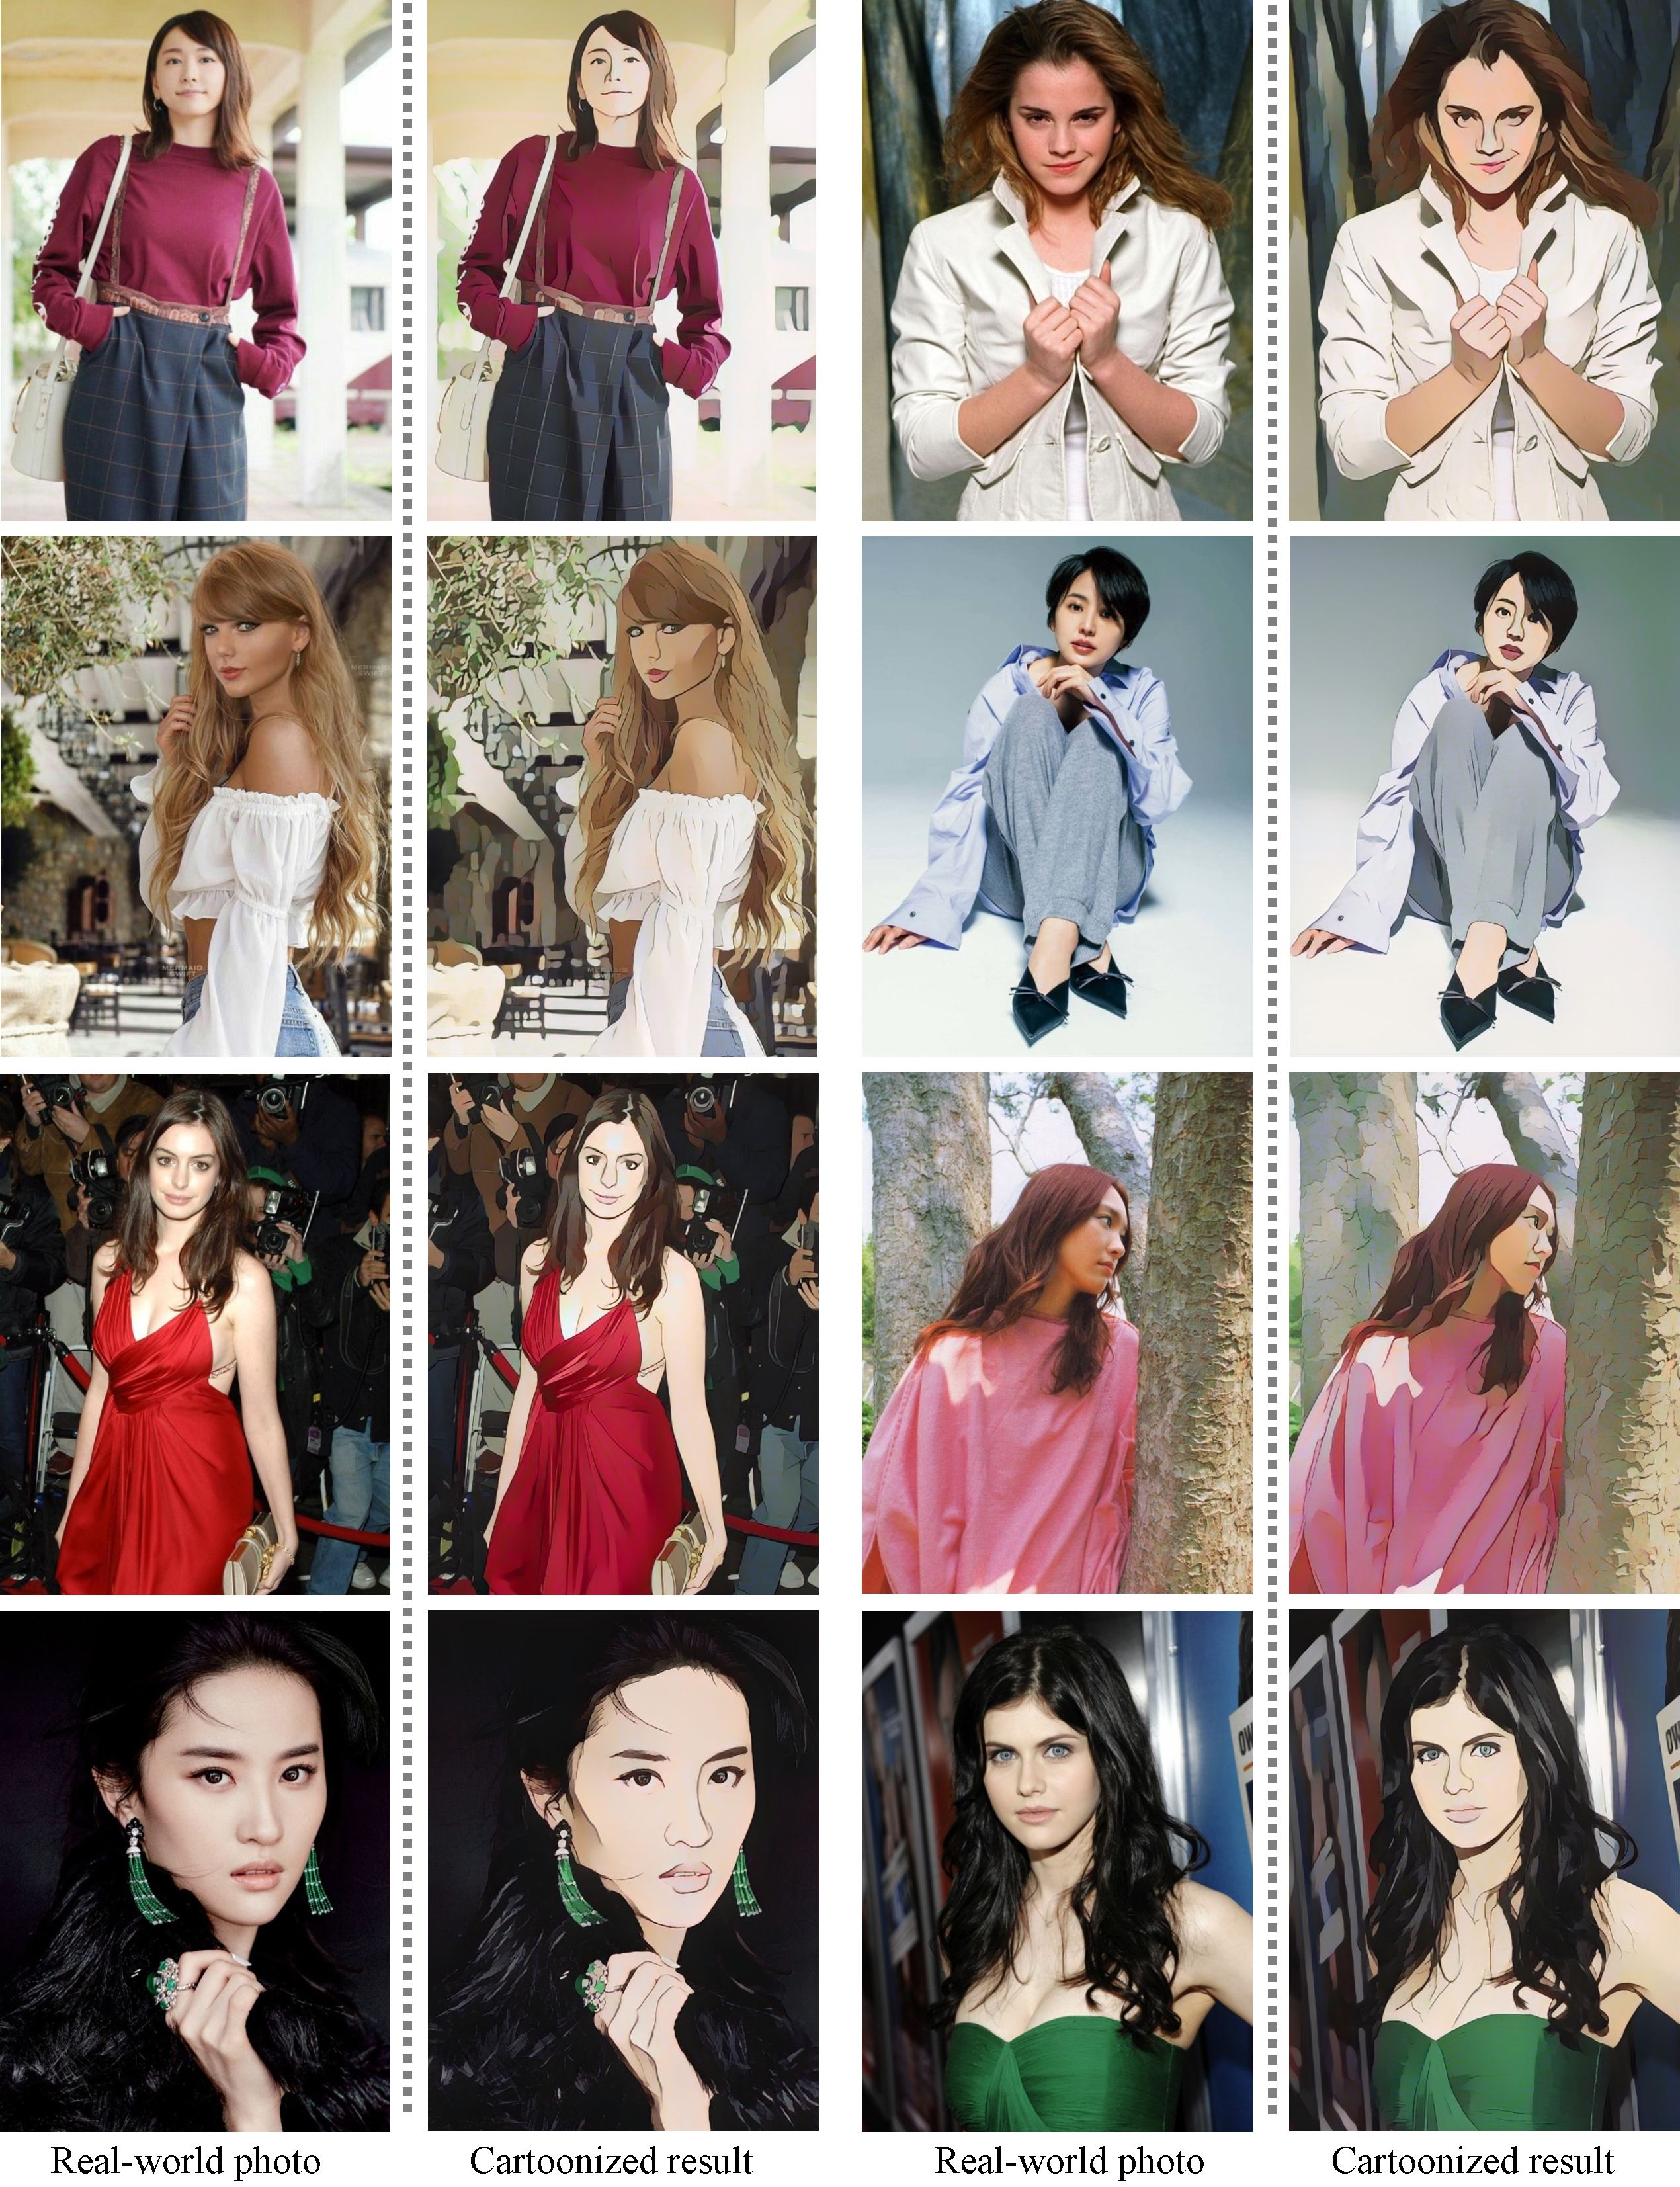
\includegraphics[width=\linewidth]{figures/person2.pdf}
\caption{Cartoonized female Celebrities.}
\label{fig:person2}
\vspace{-0.5em}
\end{figure*}

\begin{figure*}[b]
\vspace{-0.5em}
\centering
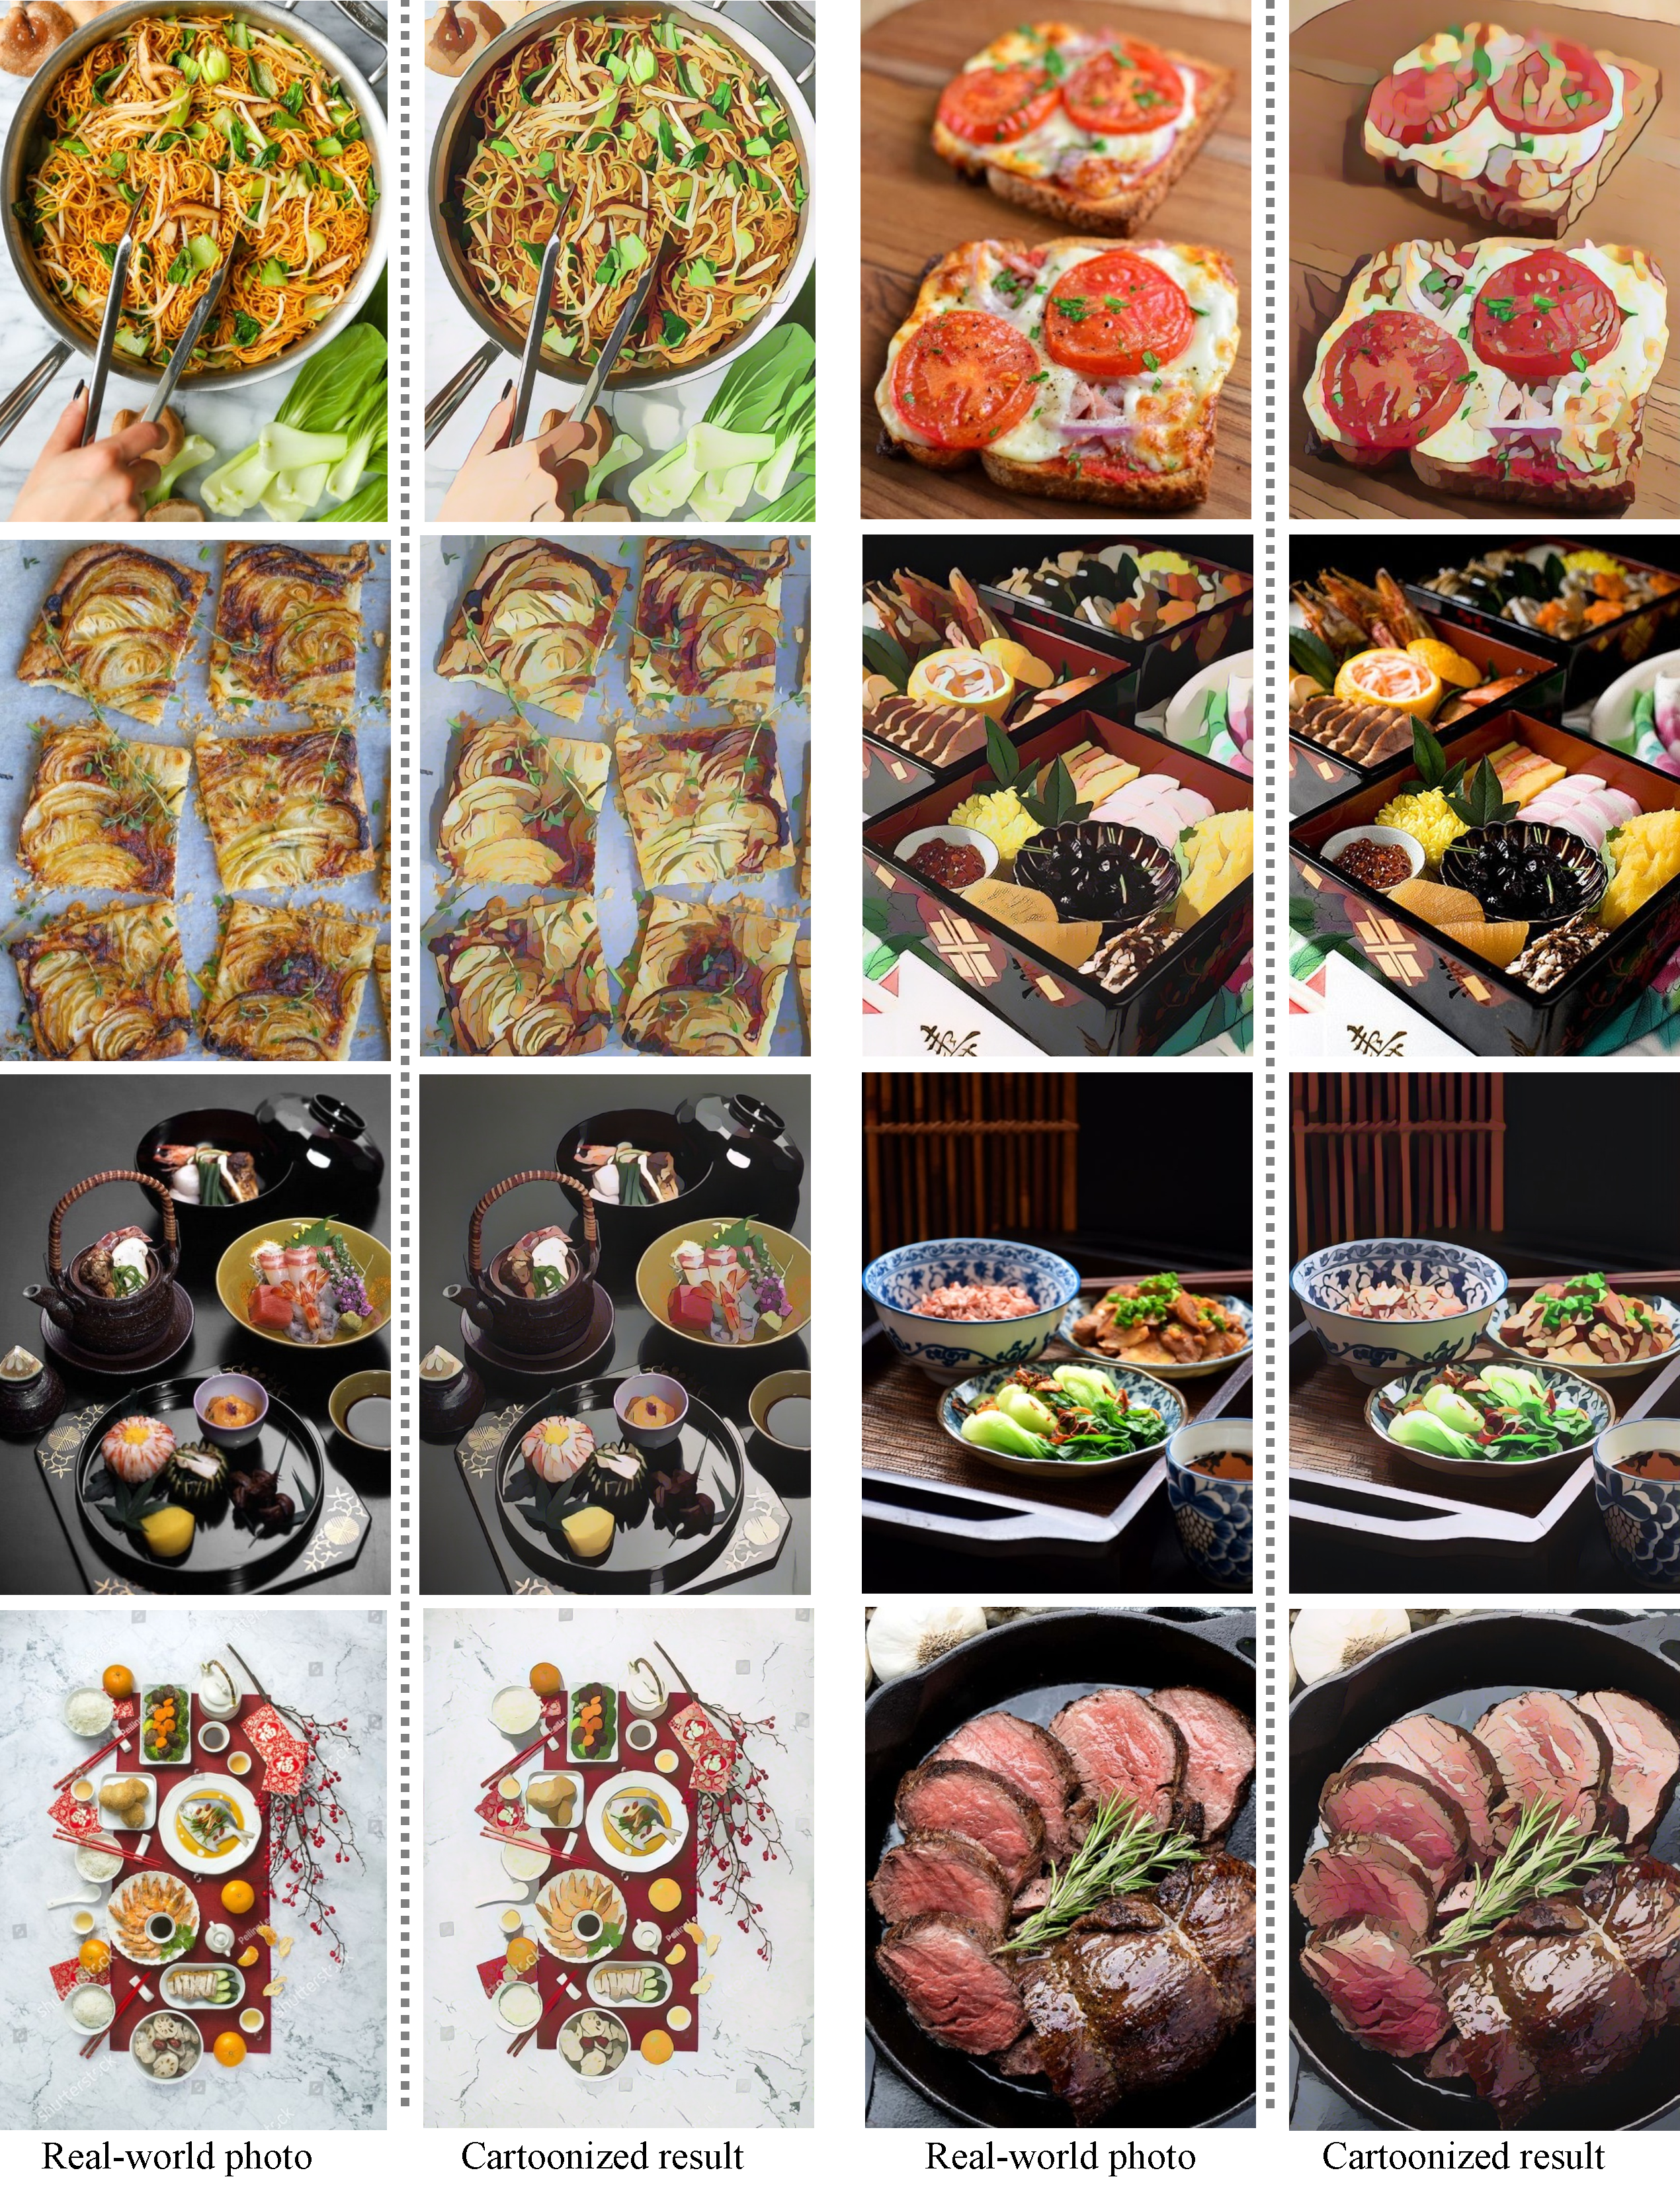
\includegraphics[width=\linewidth]{figures/food.pdf}
\caption{Cartoonized food.}
\label{fig:food}
%\vspace{-1em}
\end{figure*}

\begin{figure*}[b]
%\vspace{-1em}
\centering
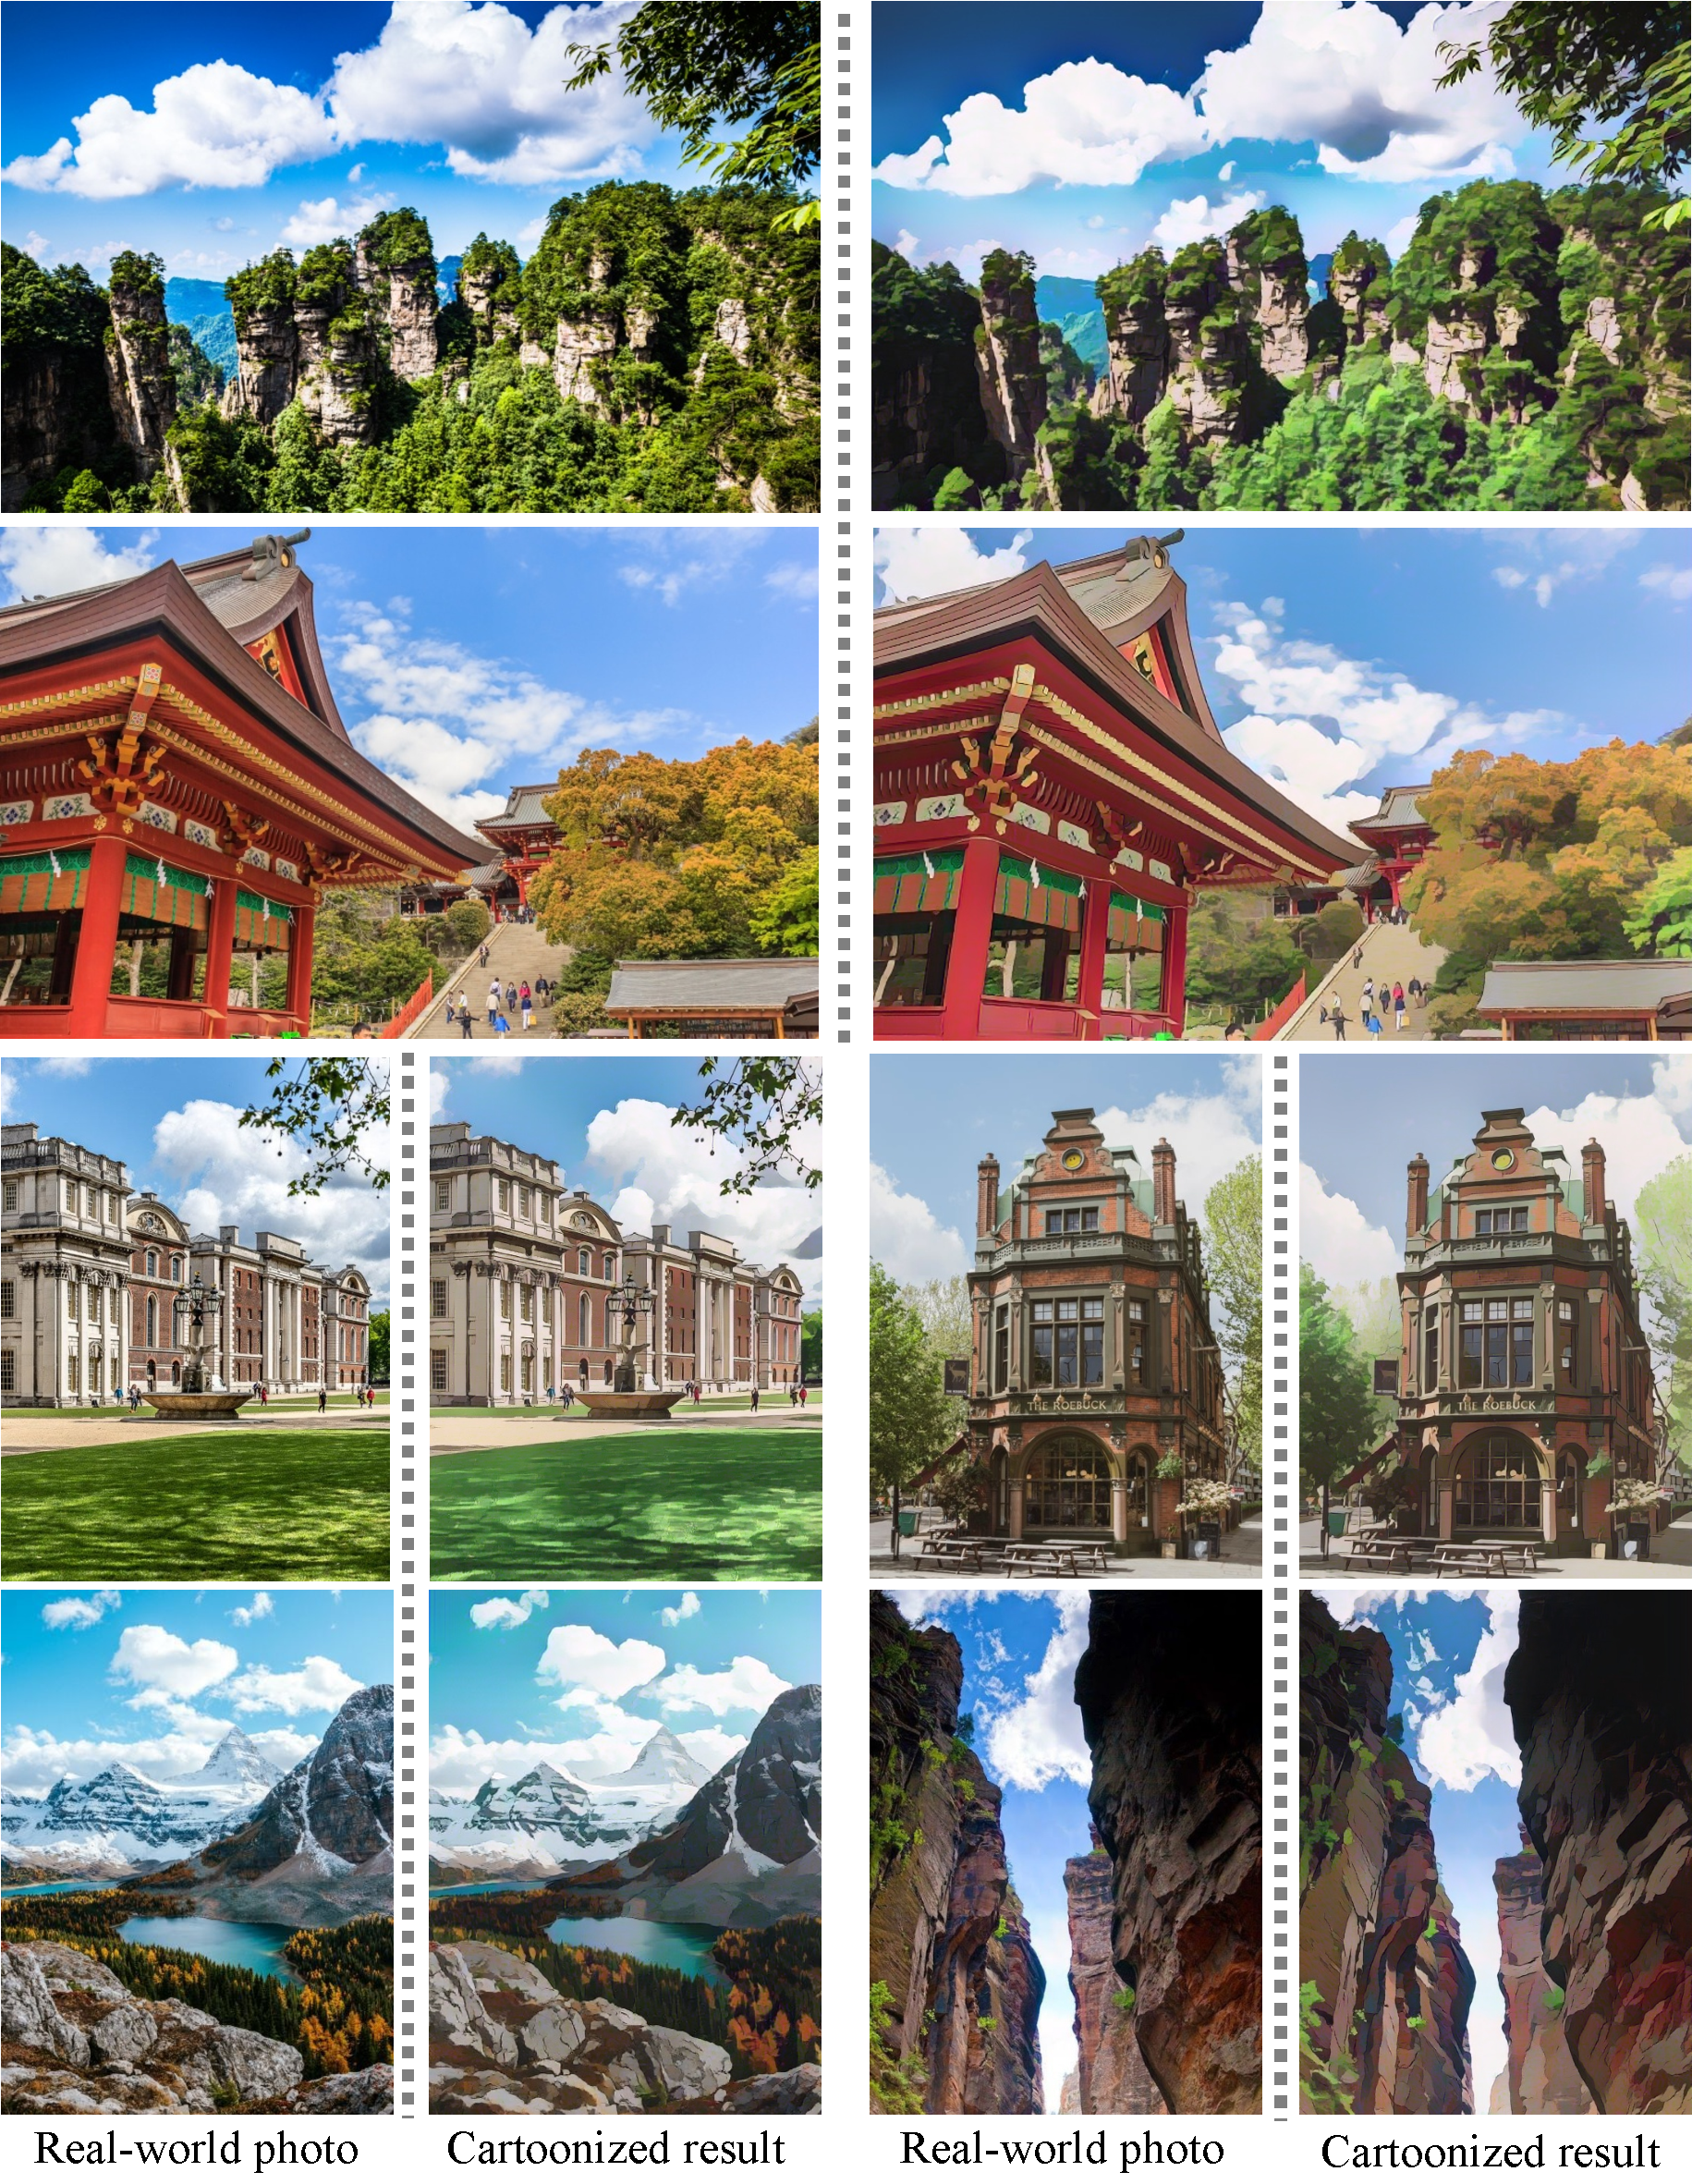
\includegraphics[width=\linewidth]{figures/scenery1.pdf}
\caption{Cartoonized scenery.}
\label{fig:scenery1}
%\vspace{-1em}
\end{figure*}

\begin{figure*}[b]
%\vspace{-1em}
\centering
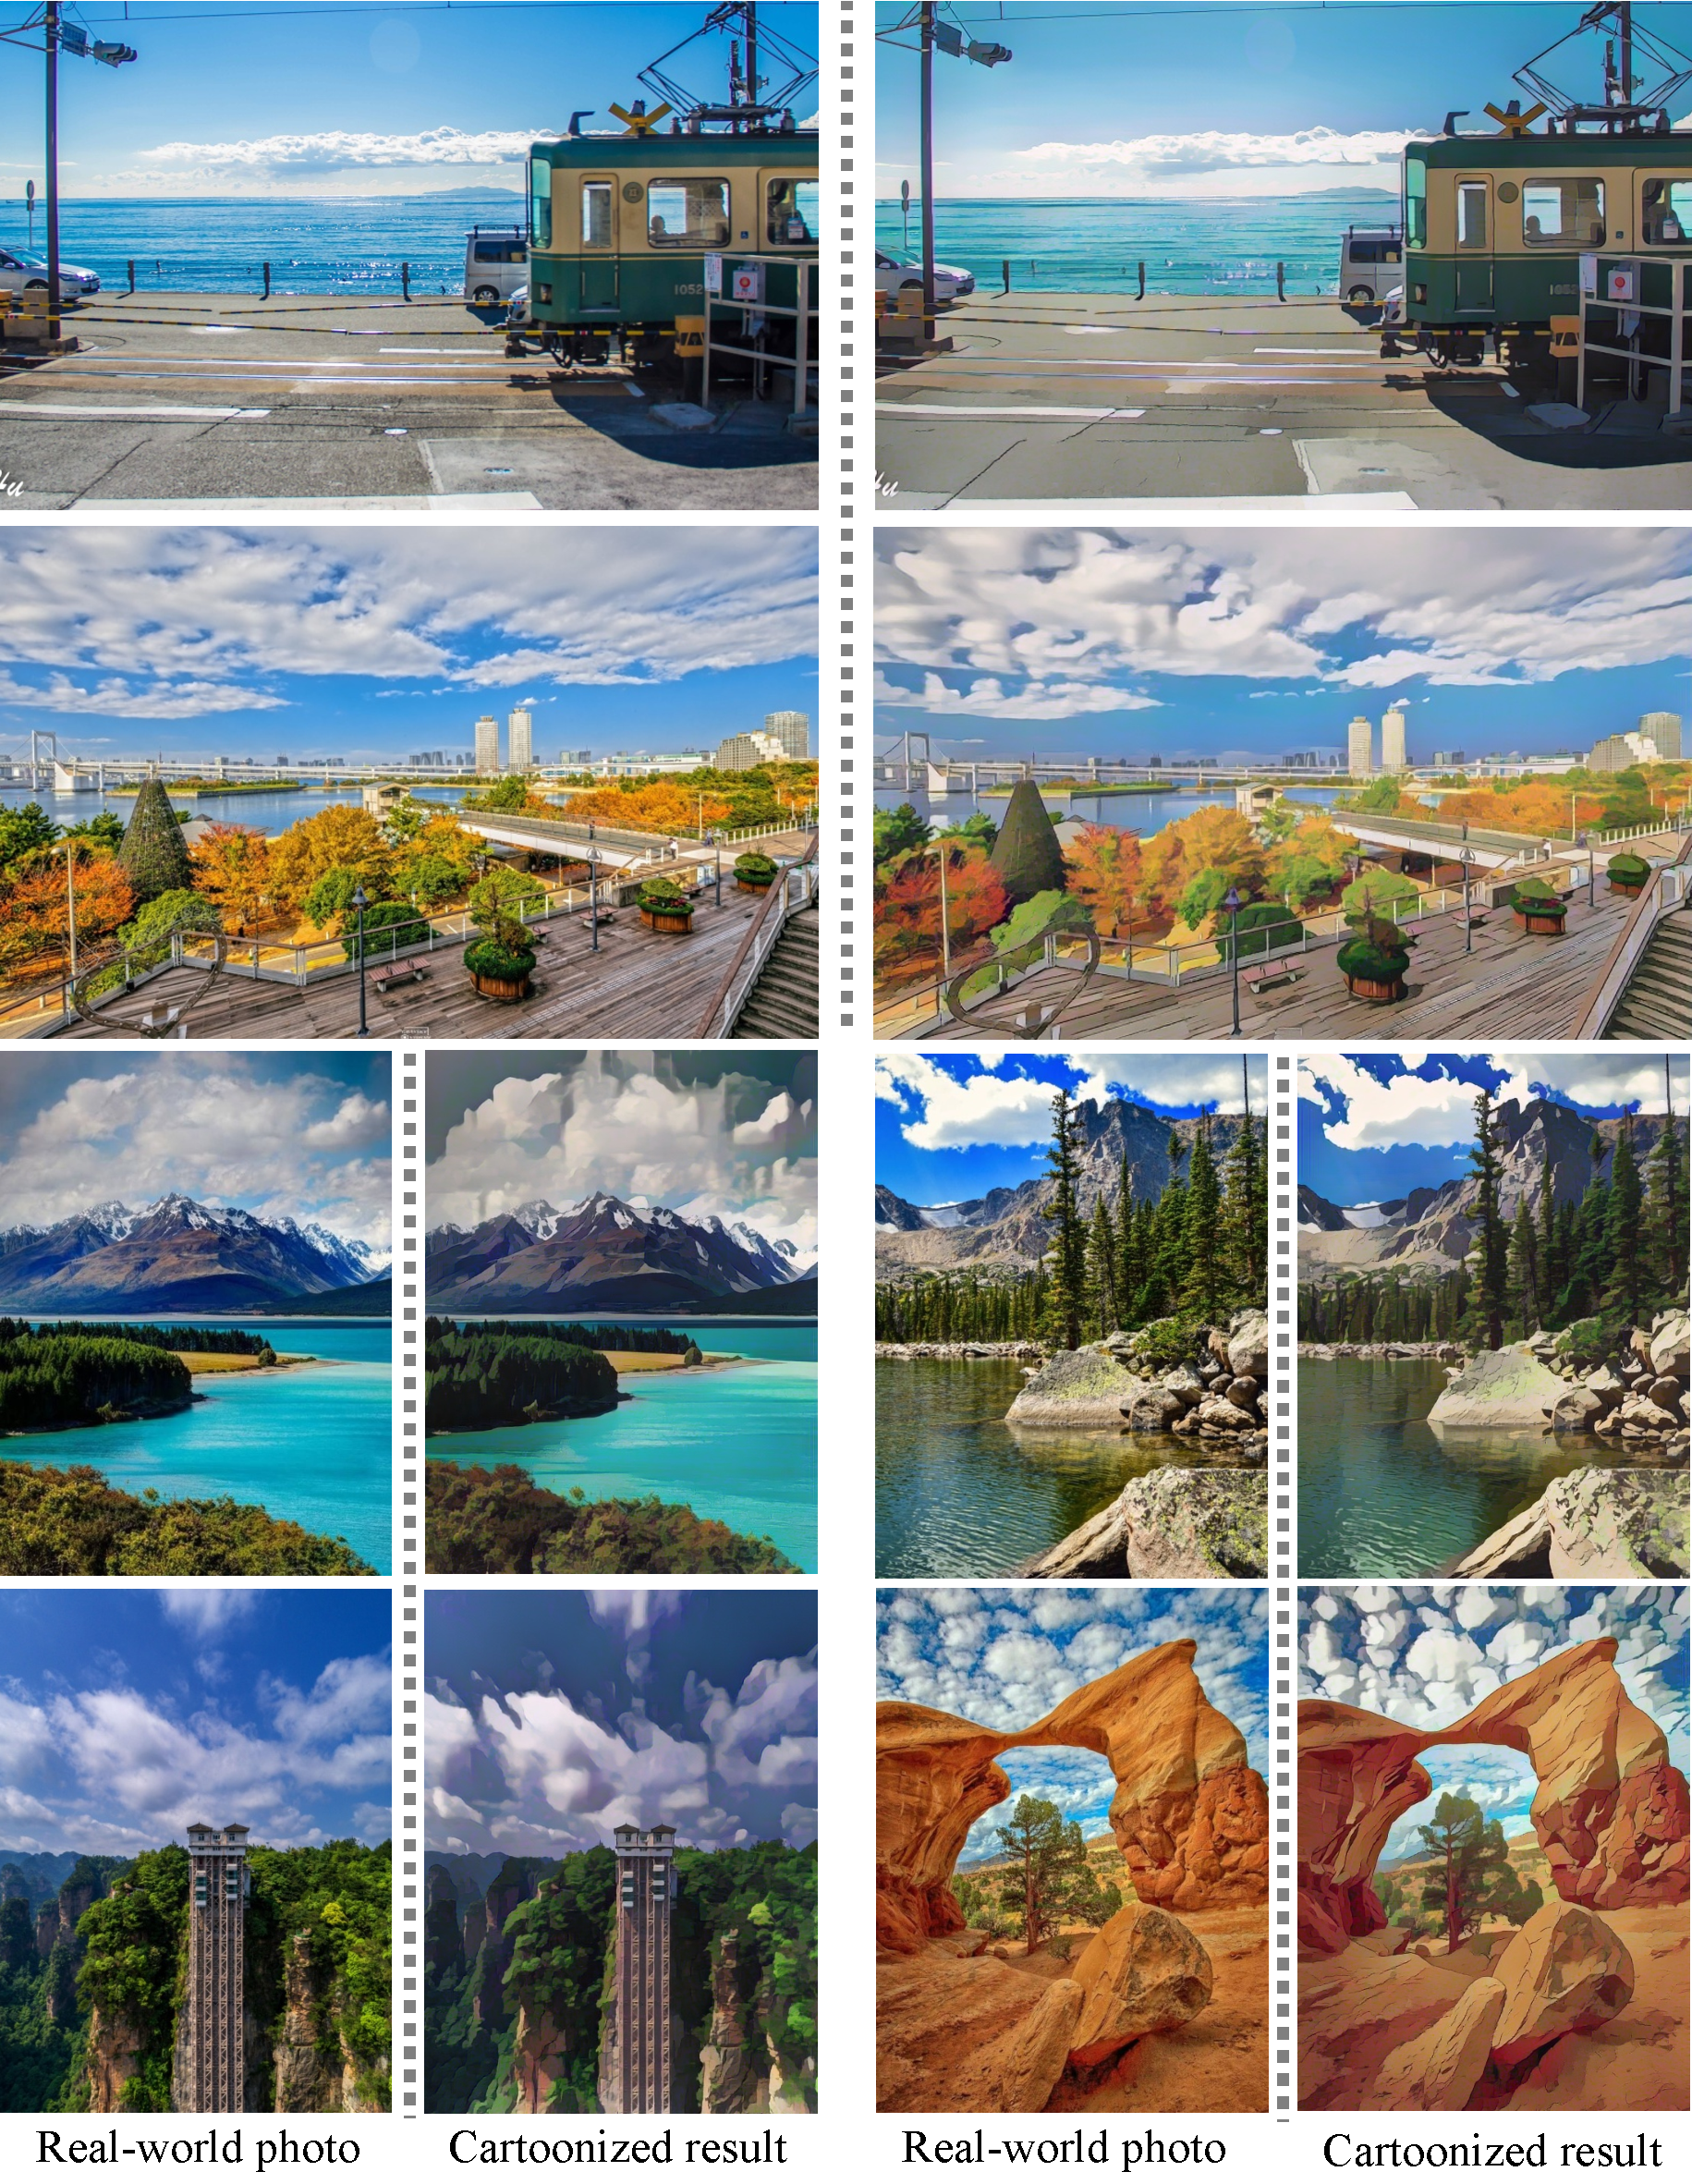
\includegraphics[width=\linewidth]{figures/scenery2.pdf}
\caption{Cartoonized scenery.}
\label{fig:scenery2}
%\vspace{-1em}
\end{figure*}

\begin{figure*}[b]
\vspace{-0.5em}
\centering
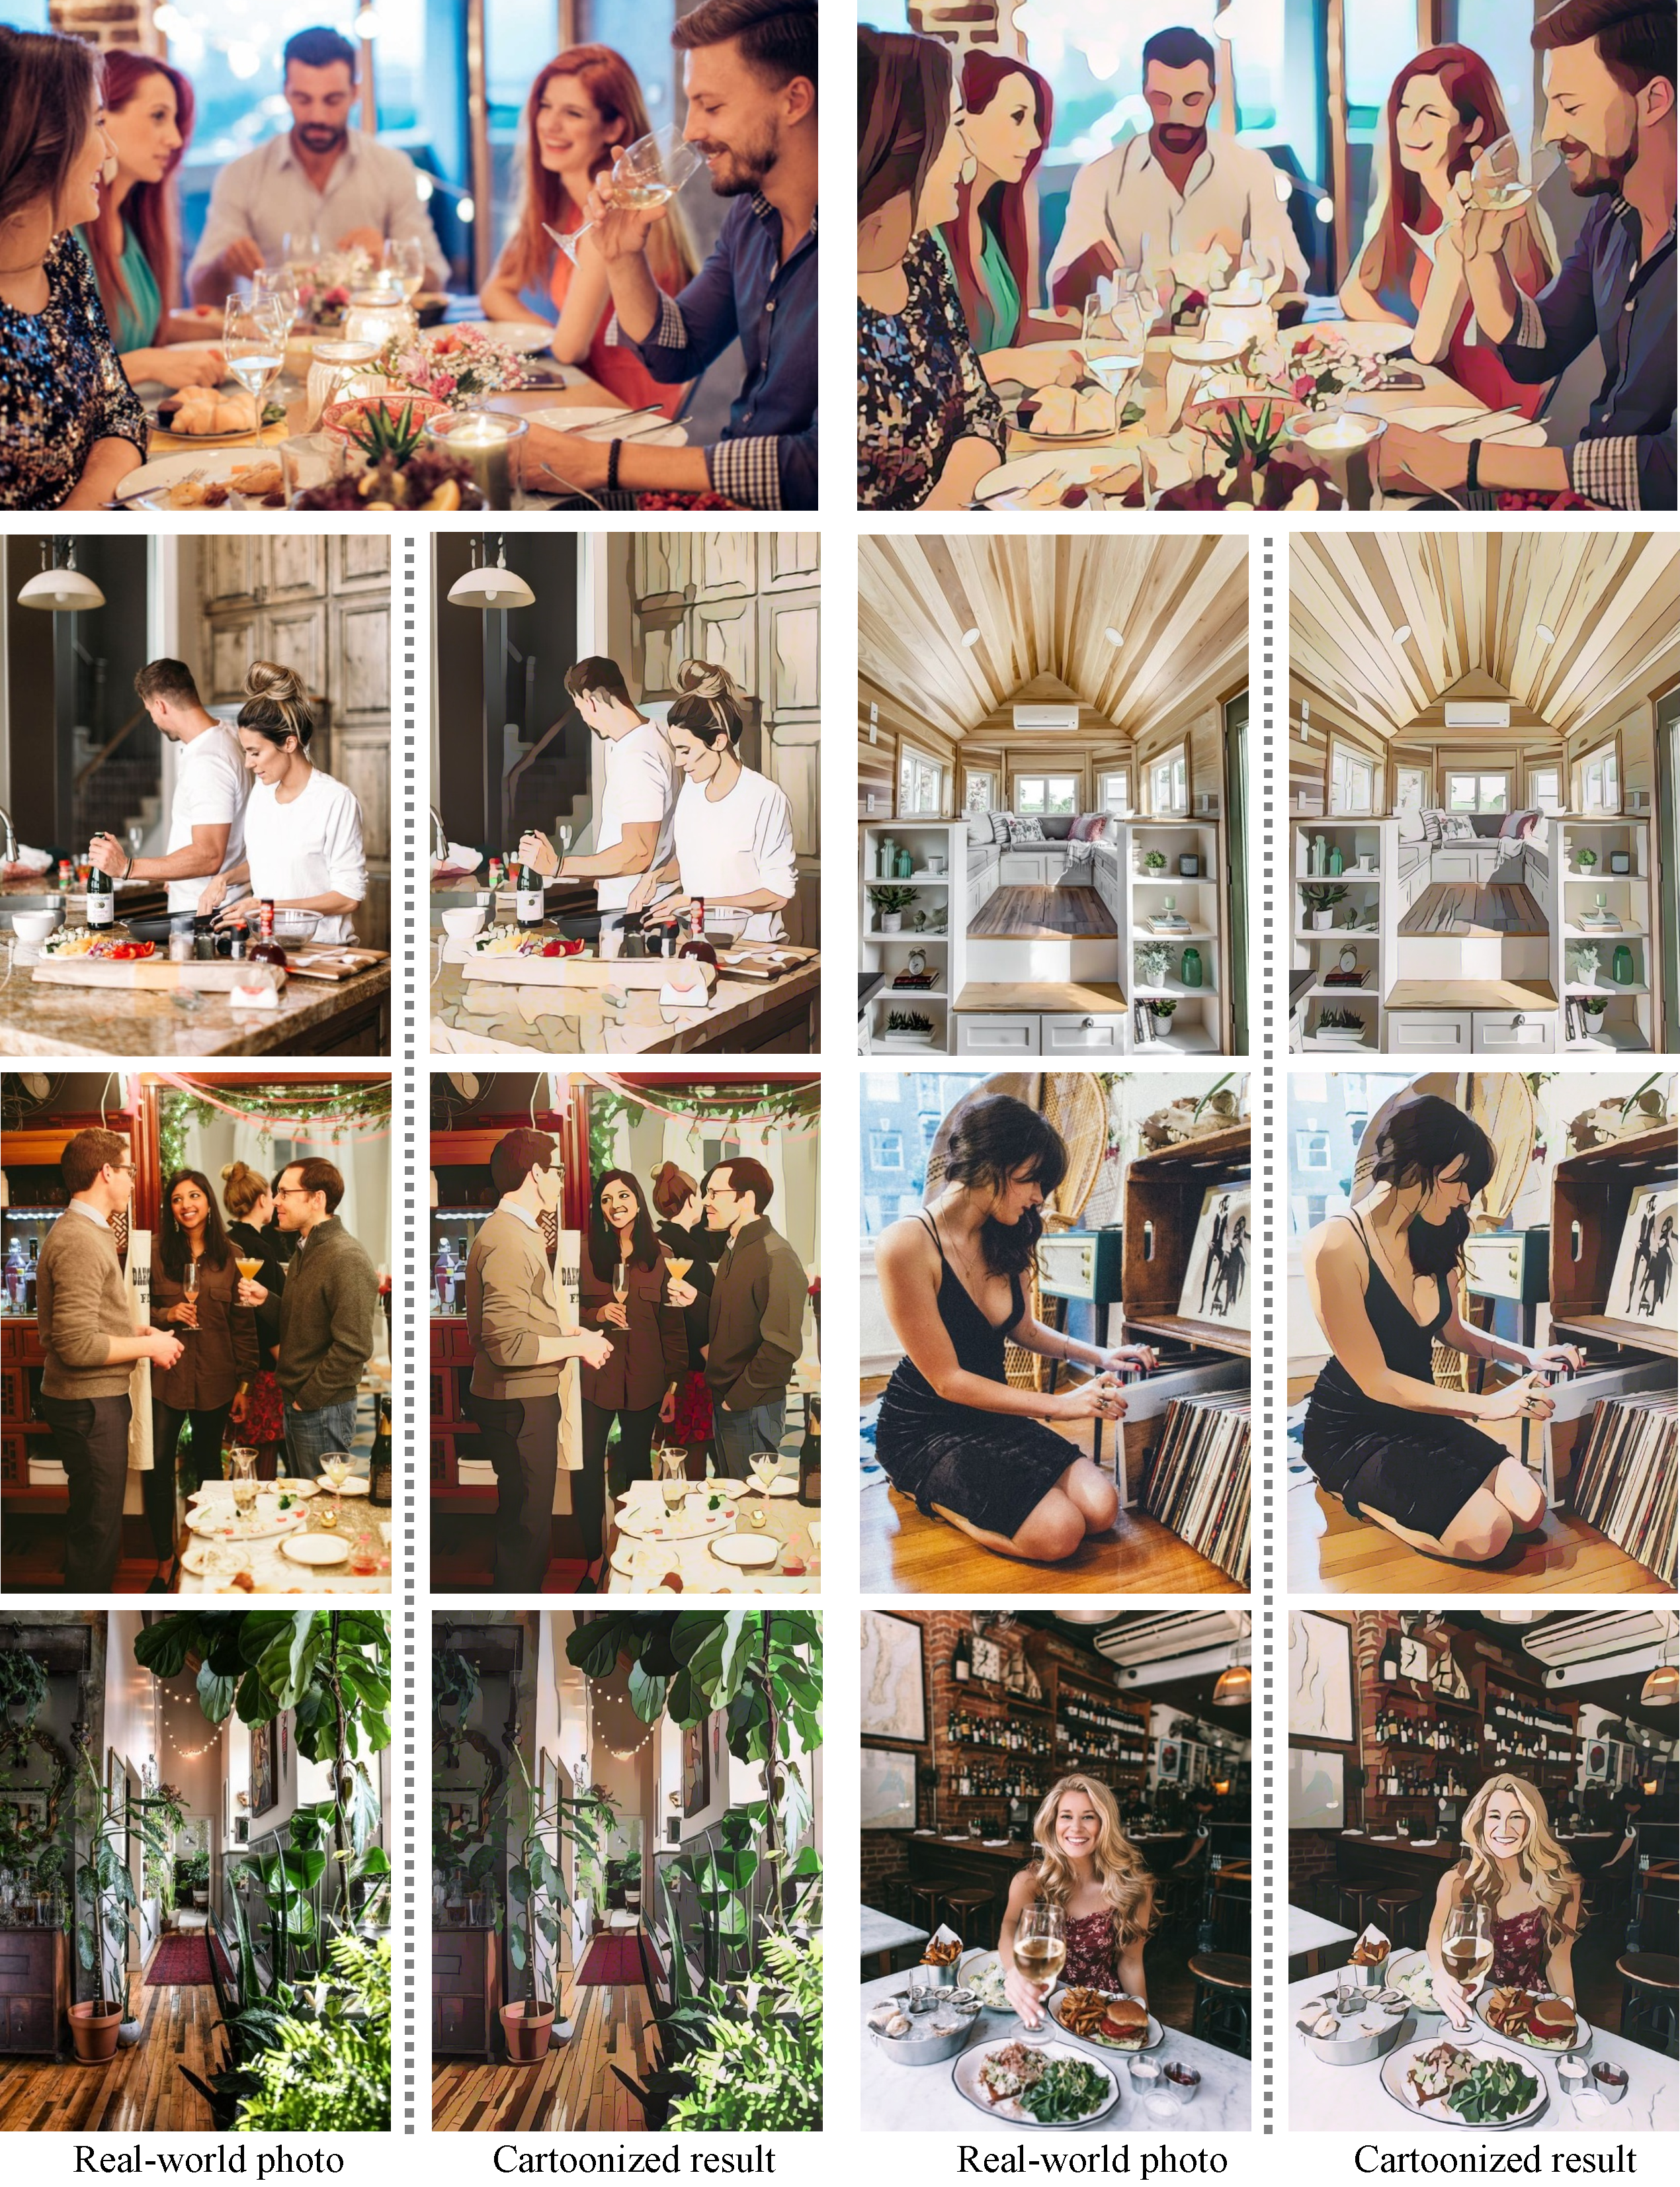
\includegraphics[width=\linewidth]{figures/home.pdf}
\caption{Cartoonized indoor scenes.}
\label{fig:home}
\end{figure*}

\begin{figure*}[b]
\vspace{-0.5em}
\centering
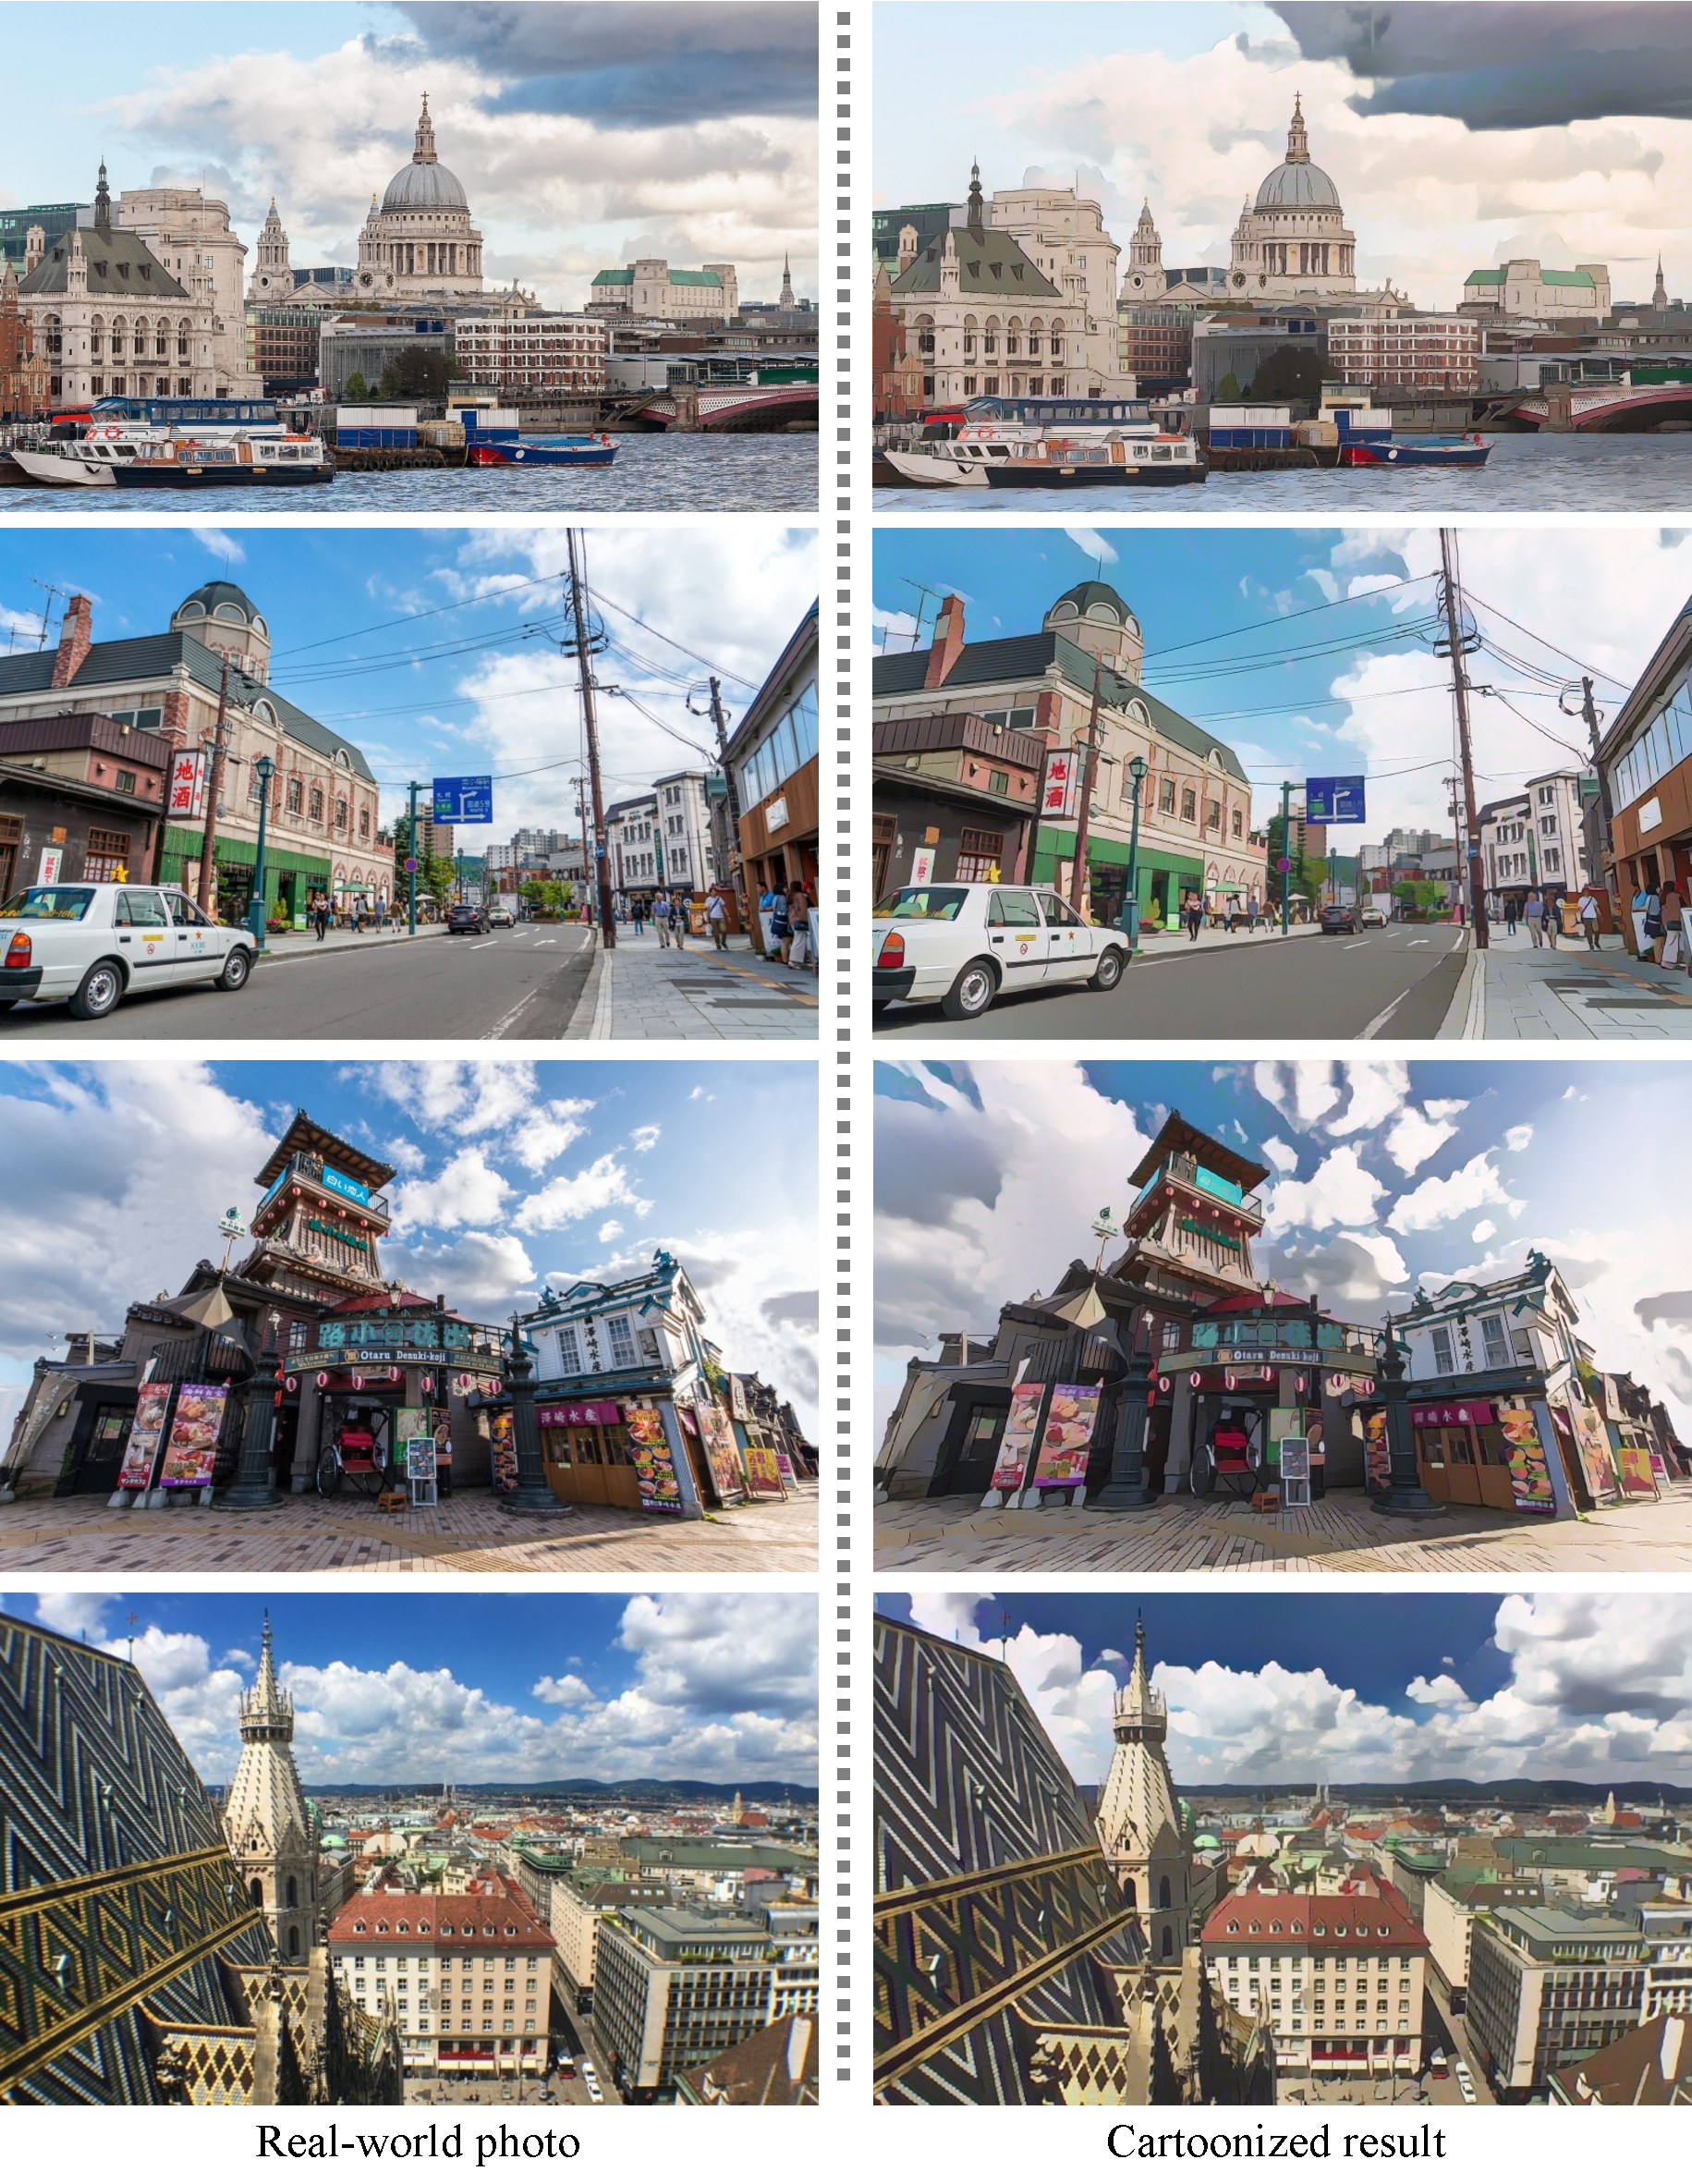
\includegraphics[width=\linewidth]{figures/city1.pdf}
\caption{Cartoonized city scenes.}
\label{fig:city1}
\end{figure*}

\begin{figure*}[b]
\vspace{-0.5em}
\centering
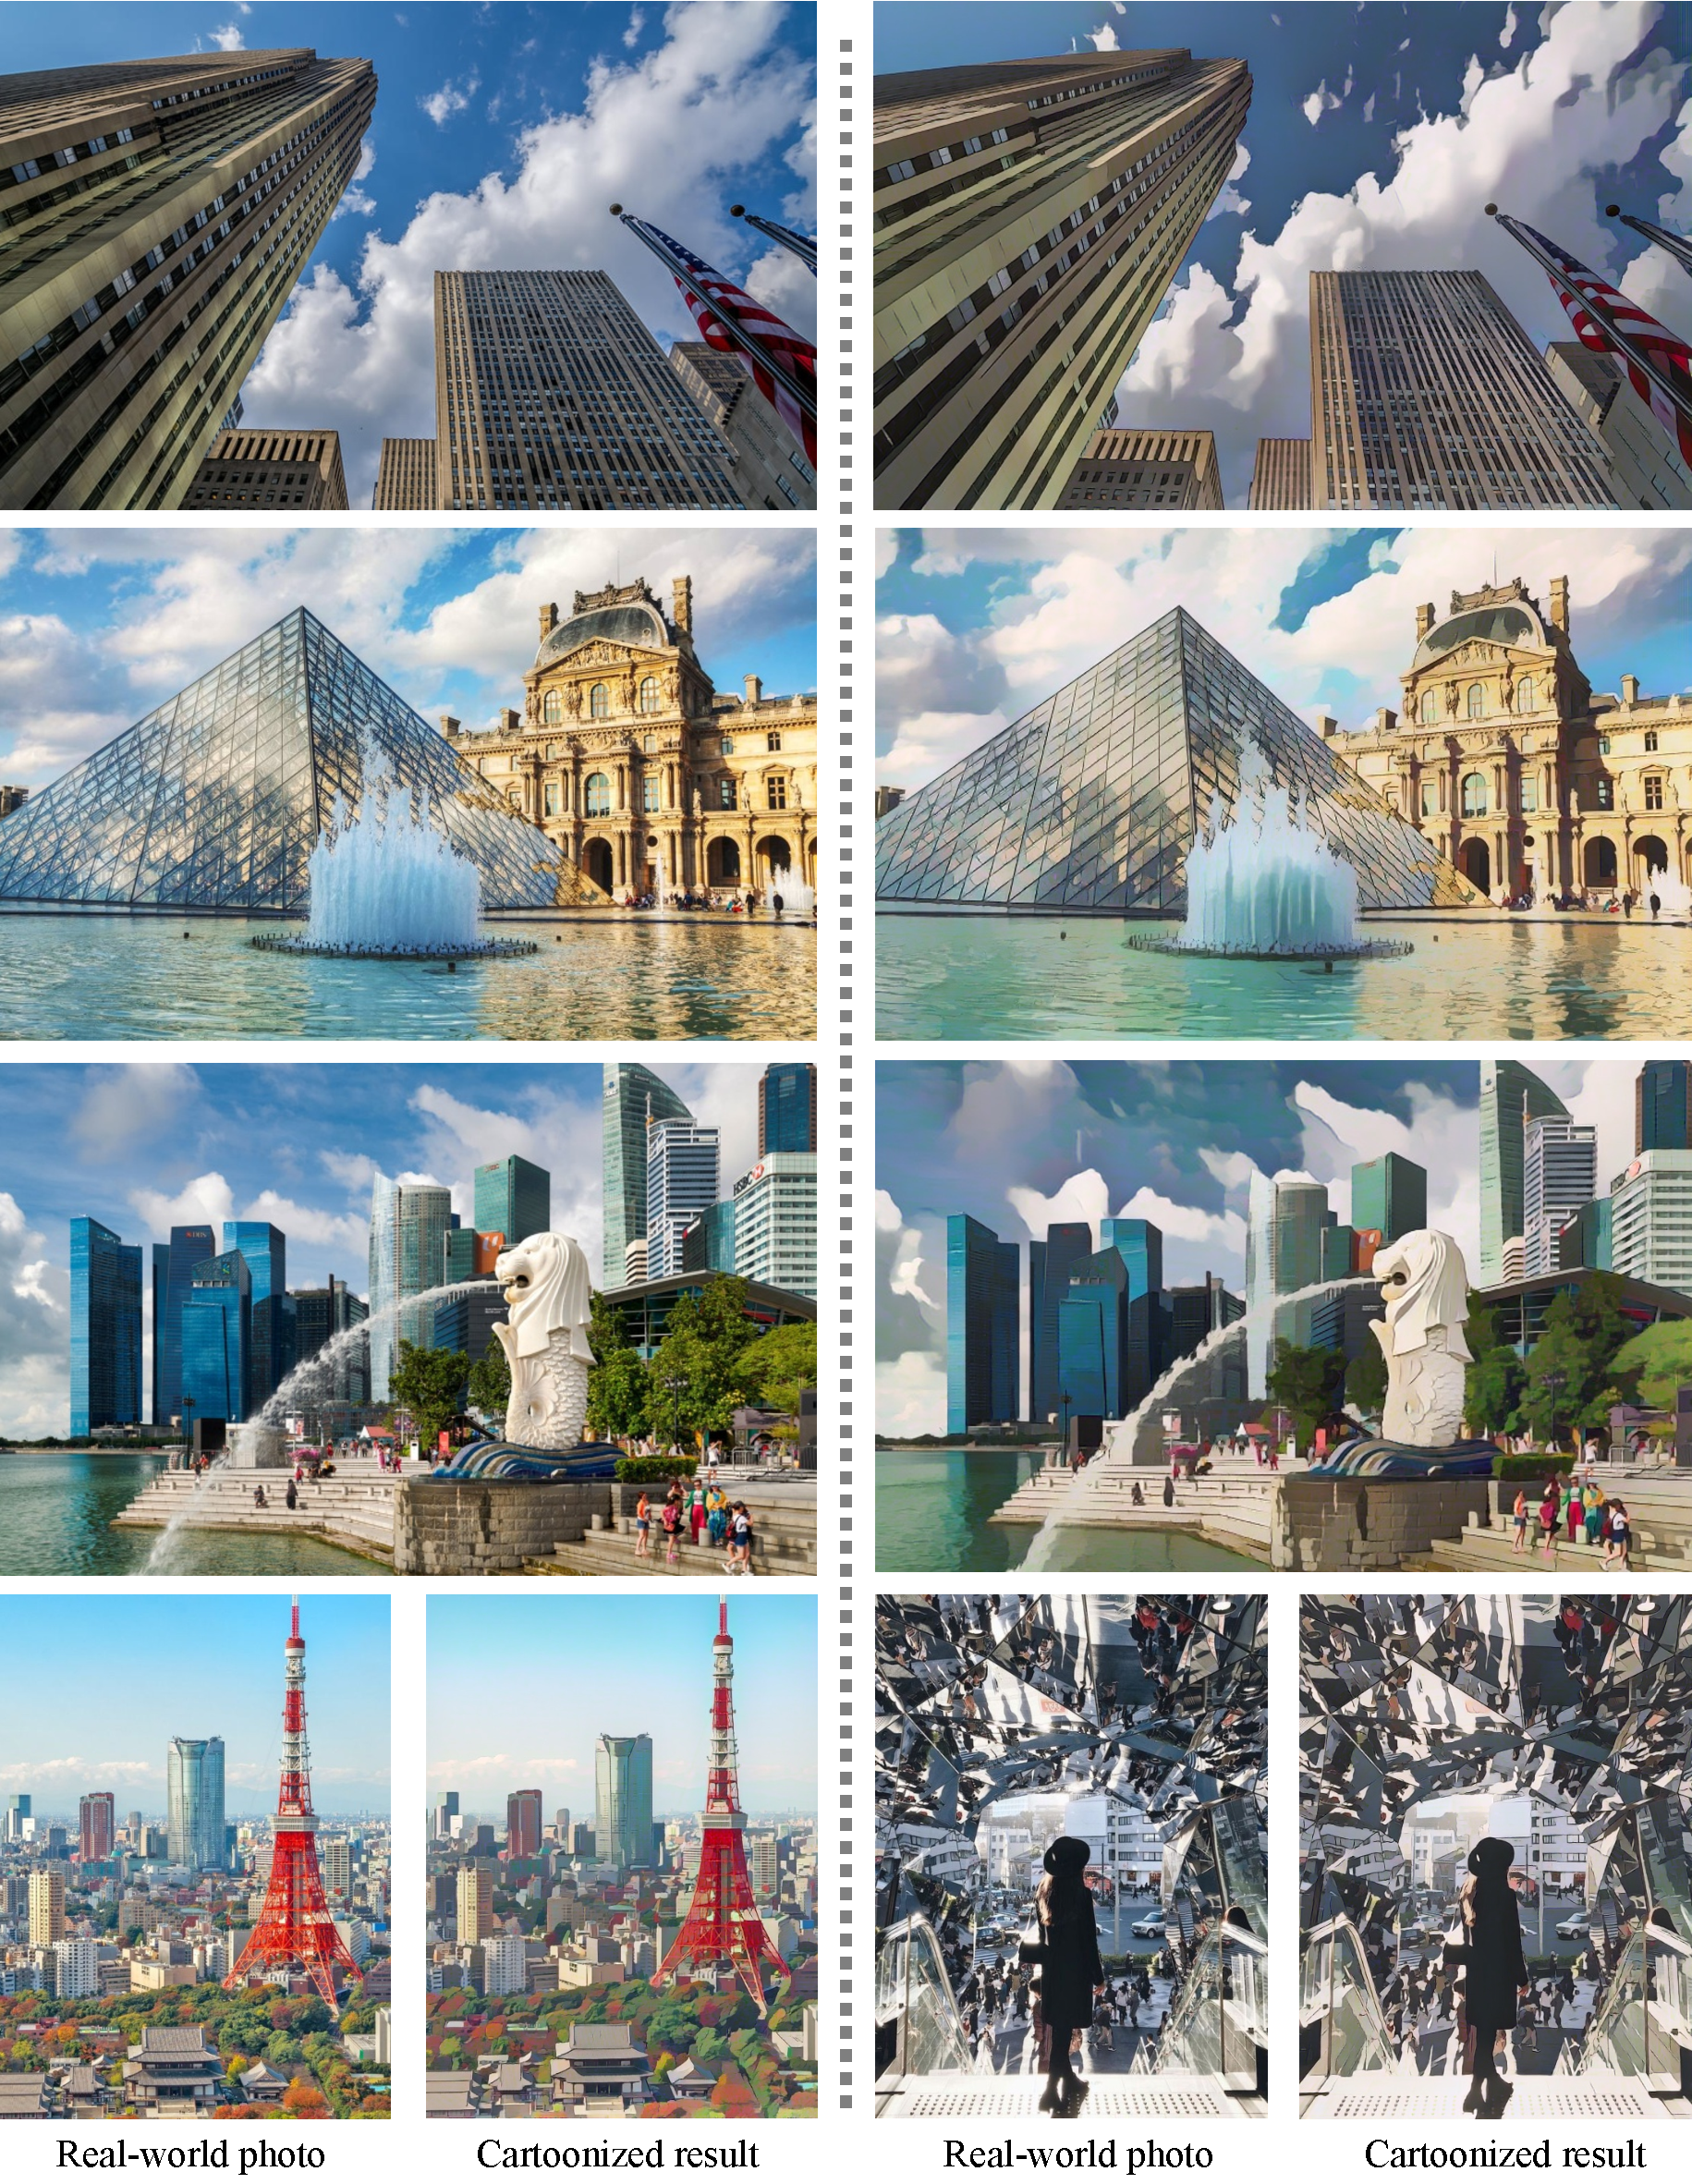
\includegraphics[width=\linewidth]{figures/city2.pdf}
\caption{Cartoonized city scenes.}
\label{fig:city2}
\end{figure*}

\begin{figure*}[b]
\vspace{-0.5em}
\centering
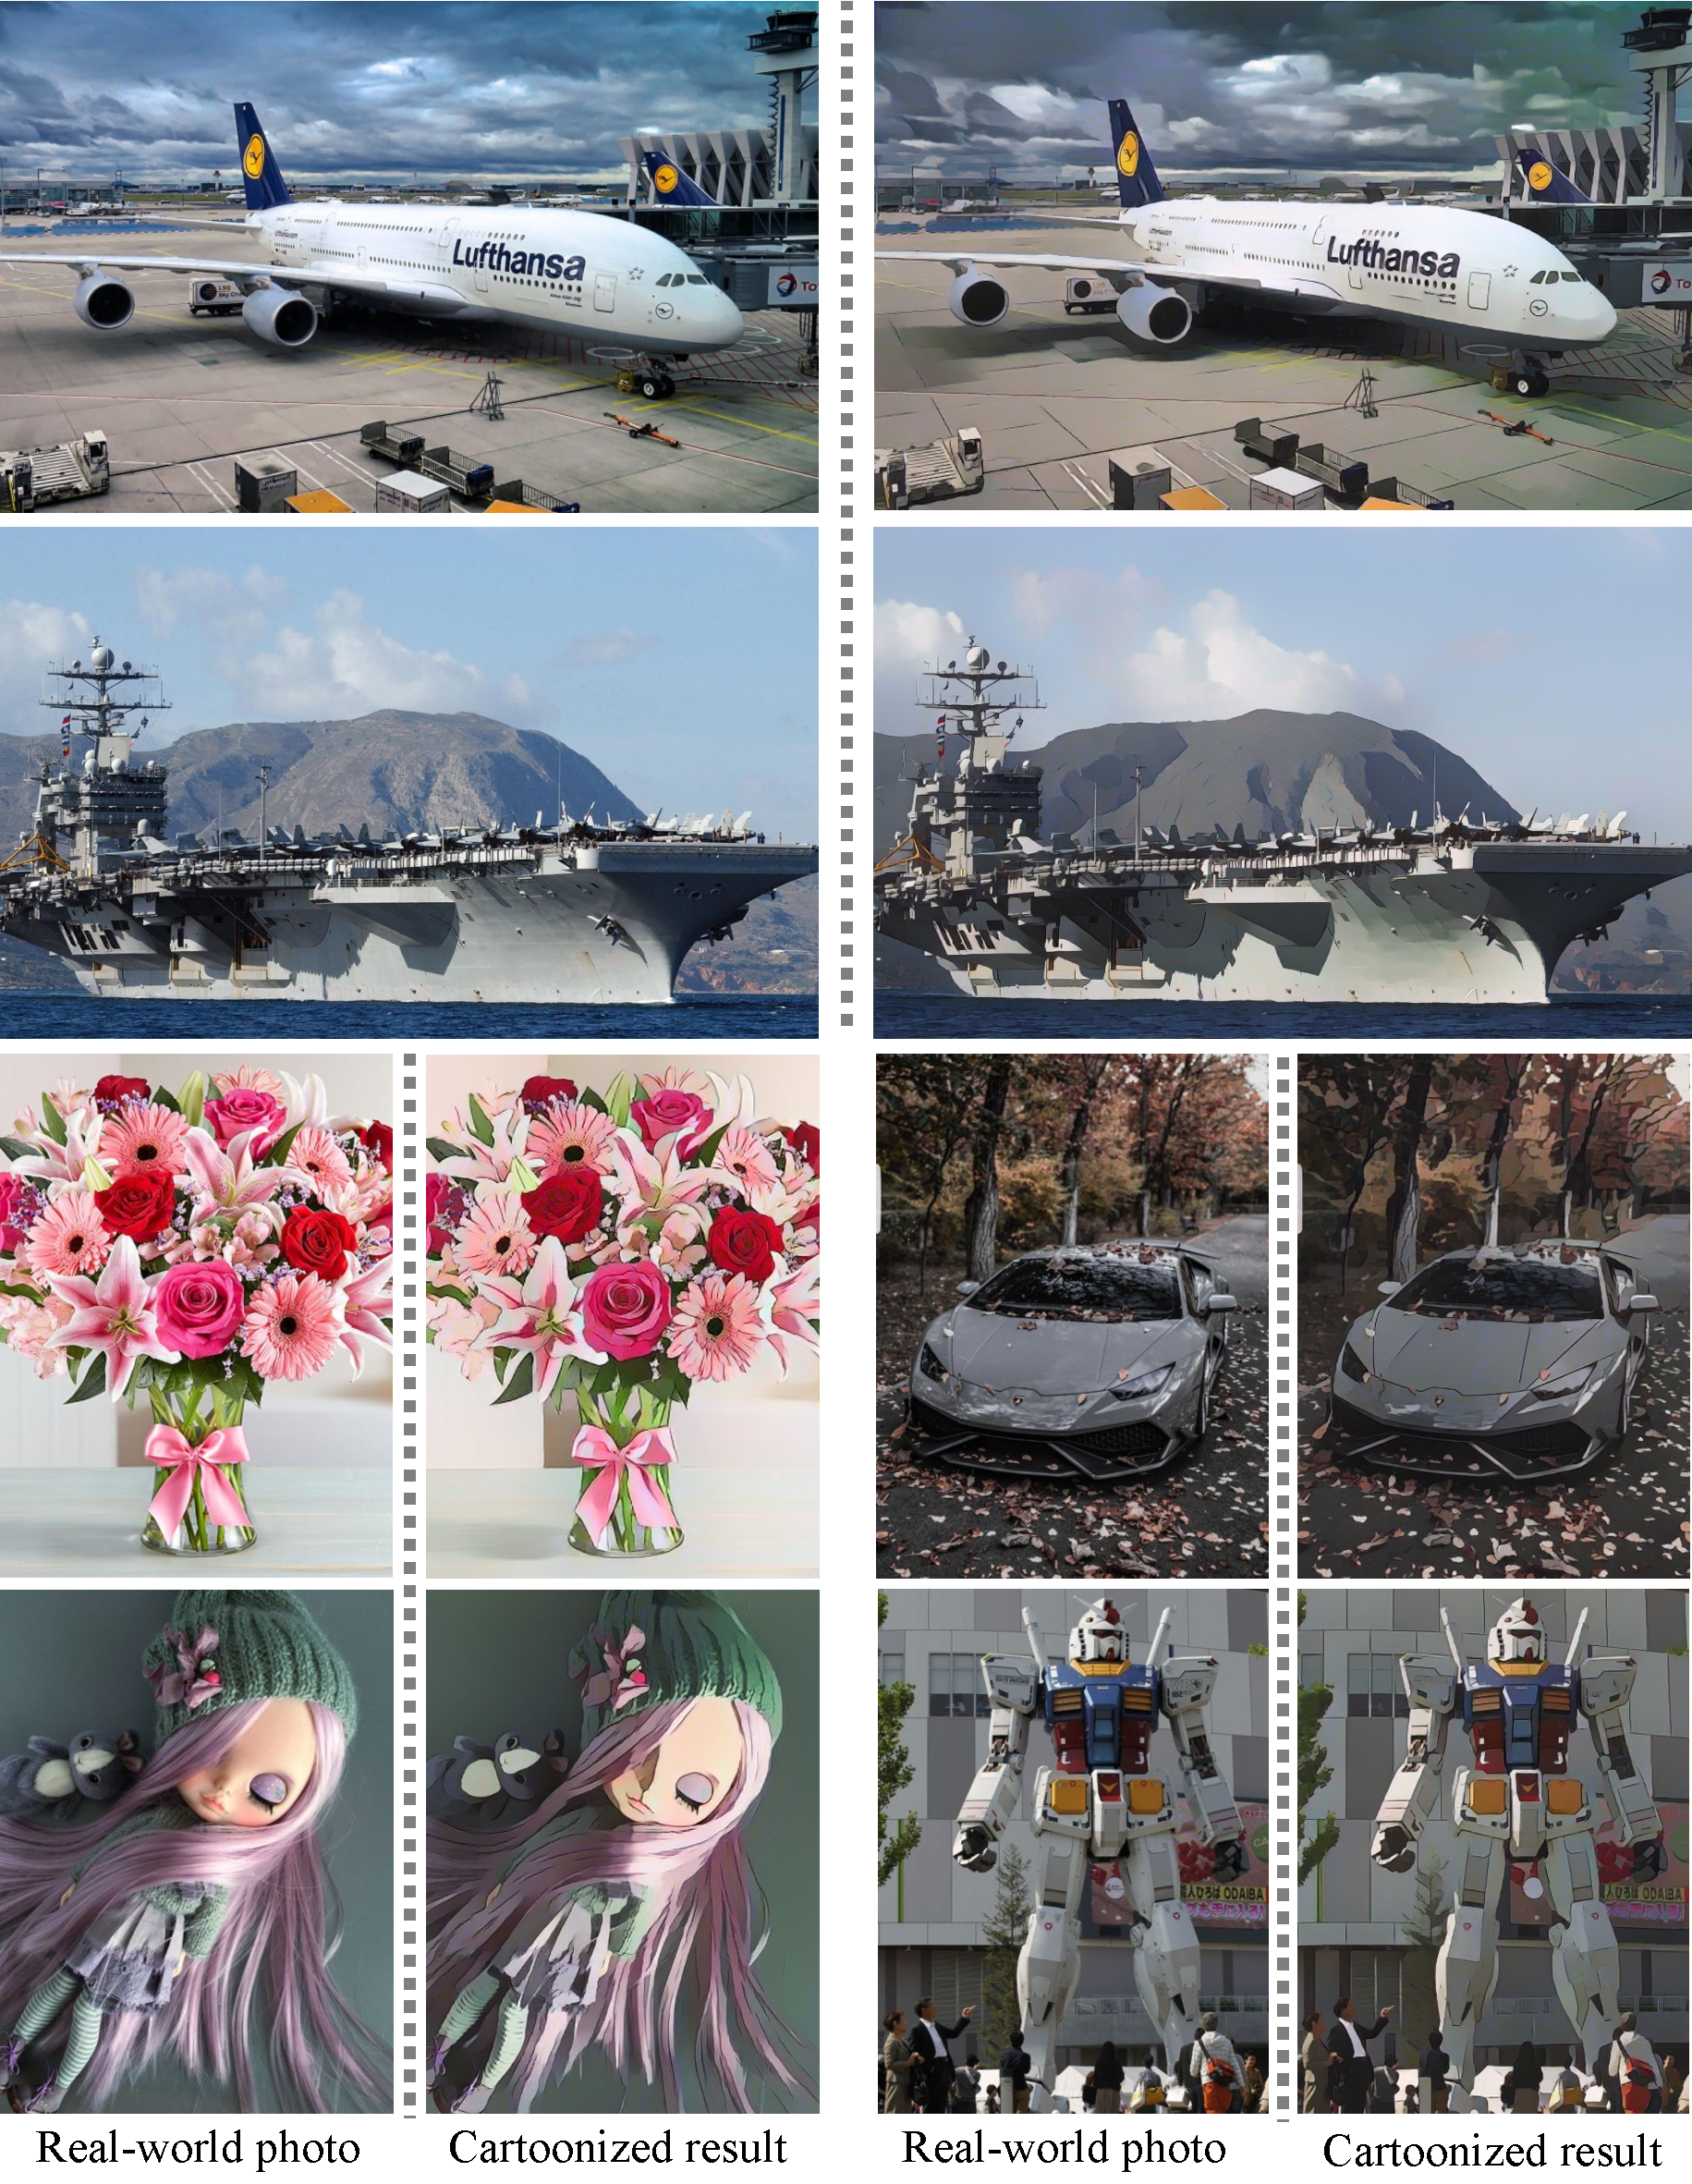
\includegraphics[width=\linewidth]{figures/object.pdf}
\caption{Cartoonized different objects.}
\label{fig:city2}
\end{figure*}

\clearpage

{\small \bibliographystyle{ieee_fullname} \bibliography{egbib}}

\end{document}
